%!TeX program = xelatex
\documentclass[12pt,hyperref,a4paper,UTF8]{ctexart}
\usepackage{zjureport}
\usepackage{graphicx} % 引入图形宏包
\usepackage{amsmath}
\usepackage{tikz}
\usetikzlibrary{shapes, arrows.meta}

\usepackage{soul, color, xcolor}
\usepackage{geometry}
\usepackage{longtable}
\geometry{a4paper,left=2cm,right=2cm,top=2cm,bottom=2cm}
%%-------------------------------正文开始---------------------------%%
\begin{document}

%%-----------------------封面--------------------%%
\cover

%%------------------摘要-------------%%
%\begin{abstract}
%
%在此填写摘要内容
%
%\end{abstract}

\thispagestyle{empty} % 首页不显示页码

%%--------------------------目录页------------------------%%
\newpage
\tableofcontents

%%------------------------正文页从这里开始-------------------%
\newpage

%%可选择这里也放一个标题
%\begin{center}
%    \title{ \Huge \textbf{{标题}}}
%\end{center}

\section{引言}
\subsection{编写目的}
本测试报告旨在对医疗预约管理系统中评价子模块的实现进行详细测试。本文档的编写目的是为了验证软件设计阶段的成果,确保软件标识与源程序开发的一致性,并为软件测试人员、程序开发员和软件分析员提供参考。

\subsection{项目描述}
在数字化和网络化技术迅速发展的背景下,中国的医疗行业正在经历一场重大的变革。尽管一些大型医疗机构已经部署了在线预约系统,但这些系统大多仅限于机构内部使用,未能实现不同医疗机构间的互联互通。同时,中小医疗机构由于技术和资金的限制,在线服务的普及仍然有待提高。鉴于此,开发一个全面且一体化的医疗预约管理系统显得尤为迫切,这不仅能够提高医疗服务的效率,还能促进医疗资源的共享。
国内外众多在线预约诊疗服务平台的出现,为患者提供了一站式的便捷服务,包括注册、登录、查看个人信息、AI病情咨询、科室浏览、医生预约、账单提交与缴费等。此外,患者还能参与问诊评价体系,为医疗服务提供反馈,帮助提升服务质量。
在现代社会的快节奏生活中,公众对医疗服务的需求日益增长,传统的电话预约和现场排队方式已逐渐无法满足当前的需求。医疗预约管理系统利用互联网技术,使用户能够随时随地进行医疗服务预约,从而提高服务效率,减少等待时间,并改善用户体验。
本项目的目标是开发一款全面的医疗预约管理系统,为患者提供一个便捷、高效的在线医疗服务平台。该系统将支持患者进行注册登录、查看个人信息、接收AI技术提供的病情咨询服务,以及在线查看医院科室信息和预约合适的医生,从而优化就诊流程。
随着信息化时代的到来,人们对医疗服务的便捷性和个性化要求不断提升。因此,我们的系统设计特别注重用户体验,提供人性化的操作方式和多样化的功能,以满足不同患者的需求。展望未来,我们计划为系统扩展更多高级功能,如接入健康监测数据(例如心率、血压等)、提供个性化健康建议、支持语音输入创建事件等,以进一步提升医疗服务的质量和效率。

\subsection{系统概述}
随着信息技术的快速发展,公众对医疗服务的便捷性和效率有了更高的期待。为满足这些需求,我们设计并实现了一个综合性的医疗预约管理系统。系统集成了在线预约、远程问诊、账单管理、用户反馈等功能,目的是显著提升医疗服务质量和患者体验。

\subsection{测试目的}
本测试旨在验证医疗预约管理系统的评价子模块是否满足以下目标:
\begin{itemize}
	\item 验证系统功能是否符合设计说明书的要求。
	\item 确保系统性能达到预期标准,包括响应时间和并发处理能力。
	\item 检查系统安全性,包括数据加密、用户认证和访问控制。
	\item 评估系统的可维护性和可扩展性。
\end{itemize}

\subsection{测试范围}
我们的测试报告主要围绕我们小组负责开发的功能展开,测试范围包括但不限于以下模块:
\begin{itemize}
	\item 用户注册与登录
	\item 处方与病历综合查询
	\item 个人医疗信息管理
	\item 科室与医生信息介绍
	\item 医生预约与时段选择
	\item 医疗费用账单管理
	\item 电子问诊单与后续跟进
	\item 医疗服务评价
\end{itemize}

\subsection{测试方法}
在本医疗预约管理系统的评价子模块测试中,我们采用了多种测试方法,以确保软件的质量和可靠性。以下是我们所采用的测试策略:

\subsubsection*{单元测试}
单元测试是针对软件中最小的可测试部分进行的测试。我们对每个组件或模块进行测试,以验证其正确性。

\subsubsection*{集成测试}
集成测试用于验证模块间的接口和交互。我们逐步将模块集成为一个完整的系统,并测试它们之间的交互是否符合设计。

\subsubsection*{系统测试}
系统测试是在完全集成的系统中进行的,以验证系统满足所有指定的需求。

\subsubsection*{自动化与手动测试}
为了确保测试的全面性和准确性,我们结合使用了自动化测试工具和手动测试。自动化测试提高了测试效率,而手动测试则专注于那些需要人类判断的测试场景。

\subsubsection*{功能测试}
功能测试,也称为行为测试,是根据产品特性、操作描述和用户方案来测试产品的可操作行为,以确定它们是否满足设计需求。本地化软件的功能测试用于验证应用程序或网站是否能够为目标用户正确工作。

\subsubsection*{边界测试}
边界测试用于探测和验证代码在处理极端或边缘情况时的行为。

\subsubsection*{压力测试}
压力测试是软件测试的一部分,它在资源受限的条件下运行测试,以确定软件在极端条件下的表现。

\subsubsection*{接口测试}
接口测试的目的是测试系统与外部系统之间的接口,特别是数据交换、传递和控制管理过程。

\subsubsection*{边界值分析}
边界值分析是对输入或输出的边界值进行测试的一种黑盒测试方法,通常作为等价类划分法的补充。

\subsection{参考资料}
\begin{itemize}
	\item 《软件设计文档国家标准》
	\item 《软件工程项目开发文档范例》
	\item 《Software Requirements, edition 2》Karl E. Wiegers
	\item 《软件需求》刘伟琴、刘洪涛译
\end{itemize}

\subsection{测试结果}
测试结果显示,医疗预约管理系统的评价子模块在以下方面表现良好:
\begin{itemize}
	\item 功能实现:所有功能均按照设计要求实现。
	\item 性能:系统响应迅速,能够处理高并发请求。
	\item 安全性:数据加密、用户认证和访问控制均符合安全标准。
	\item 可维护性和可扩展性:系统设计模块化,便于维护和升级。
\end{itemize}
然而,测试也发现了一些需要改进的地方,具体细节见测试结果分析部分。
\section{任务概述}
\subsection{系统概述}
本项目致力于开发一款全面的医疗预约管理系统,旨在为病人提供一个便捷、高效的在线医疗服务平台。该系统不仅能够实现病人的注册登录、个人信息查看,还能够通过AI技术提供病情咨询服务,帮助病人获得专业的初步诊断和建议。此外,系统允许病人在线查看医院科室信息,根据可选时段预约合适的医生,从而优化就诊流程。

随着信息化时代的到来,人们对于医疗服务的需求日益增长,对便捷性和个性化的要求也越来越高。因此,本系统的设计注重用户体验,提供人性化的操作方式和多样化的功能,以满足不同病人的需求。未来,系统还将扩展更多高级功能,如接入健康监测数据(如心率、血压等)、提供个性化健康建议、支持语音输入创建事件等,进一步提高医疗服务的质量和效率。

\subsection{系统组成}
\subsubsection{运行环境}
本系统将在多种平台上运行,包括桌面端、移动端等,以确保广泛的可访问性。系统将支持主流的操作系统,包括但不限于Windows、macOS、Android和iOS,以便病人可以在不同的设备上无缝使用。此外,系统将采用Docker容器化技术进行部署,简化安装和配置流程,确保系统的稳定性和安全性。

\subsubsection{核心功能}

系统的核心功能包括:
\begin{itemize}
	\item 病人注册与登录:提供一个简单易用的注册和登录流程,确保病人信息的安全性。
	\item 个人信息管理:允许病人查看和更新个人健康档案,包括基本信息、病史、药物使用记录等。
	\item AI病情咨询:利用人工智能技术,为病人提供初步的病情分析和医疗建议。
	\item 科室和医生预约:提供详细的科室和医生信息,支持在线预约服务,优化病人的就诊体验。
	\item 账单管理:实现医疗费用账单的在线提交、查询和支付,简化费用处理流程。
	\item 问诊评价体系:允许病人对医疗服务进行评价,促进医疗服务质量的持续改进。
\end{itemize}

通过这些功能,系统将极大地提高医疗服务的可及性和效率,为病人带来更加人性化和便捷的医疗服务体验。

我们小组负责的是病人系统的前端项目搭建,旨在为病人提供全面、便捷的医疗服务体验,从而提高医疗服务的可及性和效率。管理员、普通用户和专业用户的不同权限和功能设置,确保了系统能够满足不同用户的需求,同时保证了系统的安全性和高效运行。

对于病人而言,系统提供的关键功能包括:
\begin{itemize}
	\item 预约挂号:病人可以通过系统进行挂号和退号操作,选择适合自己的医生和时段。
	\item 费用查询与缴纳:病人可以查询医疗费用账单,并进行在线支付,简化了缴费流程。
	\item 电子问诊单:完成问诊后,病人将收到电子问诊单,便于记录和后续跟进。
	\item 问诊评价体系:病人可以参与到问诊评价体系中,对医疗服务进行评价,帮助其他病人做出更好的选择。
	\item 查询处方与病历:病人可以在线查询医生开具的处方,并搜索相关的电子病历,方便健康管理。
\end{itemize}

通过这些功能,系统将极大地提升病人的医疗服务体验,使得医疗服务更加个性化、高效和便捷。

\subsection{用户类型与特征}
为了更好地满足不同用户的需求,本医疗预约管理系统细分了用户类型,并为每种类型提供了特定的功能。以下是用户分类及其描述的表格:

	
\begin{table}[htbp]
	\centering
	\begin{tabular}{|c|p{0.8\linewidth}|} % 使用 p{} 设置文本宽度
		\hline
		用户分类 & 描述 \\
		\hline
		管理员 & 管理员是系统的超级用户,拥有最高权限,负责监控系统的日常运营、维护和更新。管理员可以管理所有用户信息、配置系统设置、审批特殊请求以及处理系统异常。 \\
		\hline
		普通用户 & 普通用户是基本模式下的使用者,享有系统提供的基础功能,如预约挂号、查看个人健康信息、接收基本的提醒通知以及地点提醒等。此分类适合不需要高级功能的日常用户。 \\
		\hline
		专业用户 & 专业用户在专家模式下拥有更高级的功能编辑权限。除了基本功能外,专业用户可以进行相对时间设置、添加提醒动作(包括执行代码脚本、修改系统设置等高级动作)、设置响铃和振动提醒等。此分类适合需要定制化服务和更多控制权的高级用户。 \\
		\hline
	\end{tabular}
	\caption{用户类型与特征}
\end{table}


\subsection{系统假设}
为了确保医疗预约管理系统能够有效地服务于病人,我们基于以下假设进行系统设计:

\begin{itemize}
	\item \textbf{用户能力假设}: 假设所有使用本系统的病人均具备操作智能手机或计算机的基本技能,并且有明确的需求进行医疗服务的预约和咨询。
	\item \textbf{技术环境假设}: 假设服务器配置能够满足系统运行的最低要求,包括操作系统、网络环境和必要的软件支持。同时,服务器安全性良好,能够抵御外部攻击,保证系统稳定运行。
	\item \textbf{网络依赖假设}: 虽然基本的医疗服务预约功能不依赖网络连接,但是部分高级功能,如在线支付和电子问诊单的接收,需要稳定的网络连接。特别是地点提醒功能,完全依赖于定位服务,因此需要一个流畅的网络环境来支持。
	\item \textbf{数据准确性假设}: 在系统运行过程中,依赖的第三方API和地图定位服务提供的数据是准确和可靠的。这确保了系统能够根据准确的数据为病人提供服务。
\end{itemize}

\subsection{系统设计与实现的约束条件}

在开发医疗预约管理系统的过程中,我们遵循以下八项约束条件,以确保系统的稳定性、安全性、高效性及用户友好性。

\begin{table}[htbp]
	\centering
	\begin{tabular}{|l|p{10cm}|}
		\hline
		\textbf{约束项} & \textbf{描述} \\
		\hline
		数据存储约束 & 系统后端采用标准化的MySQL数据库作为主要的数据存储解决方案,确保数据的持久化、一致性和安全性。实施定期备份和灾难恢复计划。 \\
		网络服务吞吐约束 & 系统设计考虑了高并发用户访问,确保网络服务具备足够的吞吐量,提供快速响应的用户体验。 \\
		数据安全约束 & 采取包括数据加密、访问控制和安全审计在内的多层次安全措施,保障用户数据的完整性、保密性和可用性。 \\
		性能要求约束 & 系统应能在各种设备上快速加载,提供流畅的用户体验,包括快速的页面响应时间和高效的数据处理能力。 \\
		用户界面约束 & 界面设计简洁直观,易于导航,确保所有用户群体都能轻松使用系统的各项功能。 \\
		兼容性约束 & 系统应在主流的操作系统和浏览器上运行良好,无需特殊配置即可访问所有功能。 \\
		可扩展性约束 & 系统架构设计应具备良好的可扩展性,便于未来增加新功能或升级现有功能,以适应不断变化的医疗需求。 \\
		法规遵从性约束 & 系统开发和运营需遵守所有相关的医疗保健法规和隐私政策,确保病人信息的合法处理和保护。 \\
		灾难恢复约束 & 系统应具备完善的灾难恢复计划和定期测试机制,确保在任何突发情况下系统的连续性和数据的完整性。 \\
		\hline
	\end{tabular}
	\caption{医疗预约管理系统设计与实现的约束条件}
\end{table}

通过遵循这些约束条件,我们的医疗预约管理系统将能够为病人提供一个全面、便捷的医疗服务体验,同时确保系统的长期稳定运行和用户数据的安全。

\subsection{用户文档}
为了确保用户能够有效地使用医疗预约管理系统,我们将提供三种类型的文档,以帮助用户快速熟悉系统并解决使用过程中可能遇到的问题。

\begin{itemize}
	\item \textbf{描述类文档}: 这类文档详细介绍了医疗预约管理系统的基本组成、功能、特性、接口和应用场景。描述类文档的目的是为用户提供一个全面的系统功能概览,并解释每个功能的具体用途和操作方法。
	\item \textbf{过程类文档}: 过程类文档通过分步指导用户如何首次使用系统中的特定功能。这些文档通过详细的步骤说明和图示,帮助用户理解并掌握每个功能的具体操作流程。
	\item \textbf{参考类文档}: 参考类文档按照专题组织信息,提供了深入的操作指南和功能解释。这类文档旨在为用户提供在执行特定操作或理解系统某项功能时所需的详细记录和解释,同时提供了快速的问题解决指南,以便用户能够高效地进行操作。
\end{itemize}

这些文档的目的是为病人提供一个全面、便捷的医疗服务体验,从而提高医疗服务的可及性和效率。通过这些文档,用户可以轻松地进行注册登录、查看个人信息、向AI咨询病情、查看医院科室信息、选择并预约医生、提交和查看账单、缴纳费用、以及参与问诊评价体系。

\subsection{术语表}

为了确保用户能够充分理解并有效地使用医疗预约管理系统,我们提供了以下详细的术语定义和描述,以帮助用户更好地掌握系统的关键概念和功能。

\begin{table}[htbp]
	\centering
	\begin{tabular}{|l|p{10cm}|}
		\hline
		\textbf{术语} & \textbf{详细描述} \\ \hline
		医疗预约系统 & 一个综合性的在线服务平台,旨在为病人提供便捷的医疗服务预约体验。它允许用户远程预约挂号、查询医疗费用、查看电子问诊单据、评价医疗服务质量,并通过数据分析优化医疗资源分配。 \\ \hline
		注册登录 & 病人在使用医疗预约管理系统前必须进行的账户创建和身份验证过程。这确保了用户信息的安全性和隐私保护,同时为用户提供个性化的医疗服务。 \\ \hline
		AI咨询 & 利用先进的人工智能技术,系统提供初步的病情分析和健康建议服务。AI咨询能够根据病人提供的症状信息,给出可能的疾病诊断和建议的下一步行动。 \\ \hline
		科室浏览 & 系统提供的一个功能,允许病人查看医院内不同科室的详细信息,包括科室的专业领域、医生团队介绍和特色服务,以便病人能够根据自身需求选择合适的医疗服务。 \\ \hline
		预约挂号 & 病人可以通过系统选择心仪的医生和方便的时段进行预约。此功能通过智能排队和时间管理机制,最大化地减少病人的等待时间,提高就诊效率。 \\ \hline
		账单管理 & 一个集成在系统中的功能,使病人能够轻松查询、提交和支付医疗费用账单。账单管理功能支持多种支付方式,并提供详细的费用明细,以便病人了解费用构成。 \\ \hline
		电子问诊单 & 问诊结束后,病人将收到一份包含诊断结果、治疗建议和处方信息的电子文档。电子问诊单便于病人随时查看和保存,同时也为医生后续的跟踪治疗提供了便利。 \\ \hline
		问诊评价体系 & 医疗预约管理系统内置的评价机制,允许病人对接受的医疗服务进行评价。这些评价不仅为其他病人提供参考,也为医疗机构提供了改进服务质量的宝贵反馈。 \\ \hline
		处方查询 & 系统提供的一项功能,使病人能够在线查看医生开具的处方详情,包括药物名称、用法用量等。处方查询功能确保病人能够准确理解医嘱,并按需购买药品。 \\ \hline
		病历搜索 & 病人可以通过系统搜索并访问自己的历史医疗记录和病历资料。这项功能对于病人了解自己的健康状况、跟踪疾病进展和预防措施具有重要意义。 \\ \hline
	\end{tabular}
	\caption{医疗预约管理系统关键术语表}
\end{table}

通过这些术语的明确定义,我们希望病人能够更加顺畅地使用医疗预约管理系统,享受到全面、便捷的医疗服务体验。系统的设计旨在提高医疗服务的可及性和效率,简化病人的医疗服务流程,提升整体医疗服务质量。

\newpage

\section{需求规定}
\section{功能验证测试}
由于类的实现已经包含在了功能中,因此我们不再给出单独的类(具体来说是用户类)的测试,而直接展示功能性验证的结果。由于空间有限,实际效果只展示了部分,具体的所有功能可见于表格。

\subsection{用户注册与登录}

病人可以通过注册账户并登录系统,以便安全、便捷地使用系统提供的各项服务。

\begin{table}[!h]
	\centering
	\begin{tabular}{|p{6cm}|p{6cm}|}
		\hline
		\textbf{注册} & \textbf{登录} \\
		\hline
		用户访问注册页面,填写必要信息(如用户名、密码、邮箱等),提交注册请求。 & 用户访问登录页面,输入注册时的用户名和密码。 \\
		系统验证用户提供的信息是否符合要求,若符合则完成注册,向用户发送确认邮件。 & 系统验证用户输入的用户名和密码是否匹配注册时记录的信息。 \\
		用户收到确认邮件,点击确认链接完成账户激活。 & 登录成功后,用户可以访问系统提供的各项服务。 \\
		\hline
	\end{tabular}
	\caption{用户注册与登录机制}
\end{table}

\begin{figure}[!h]
	\centering
	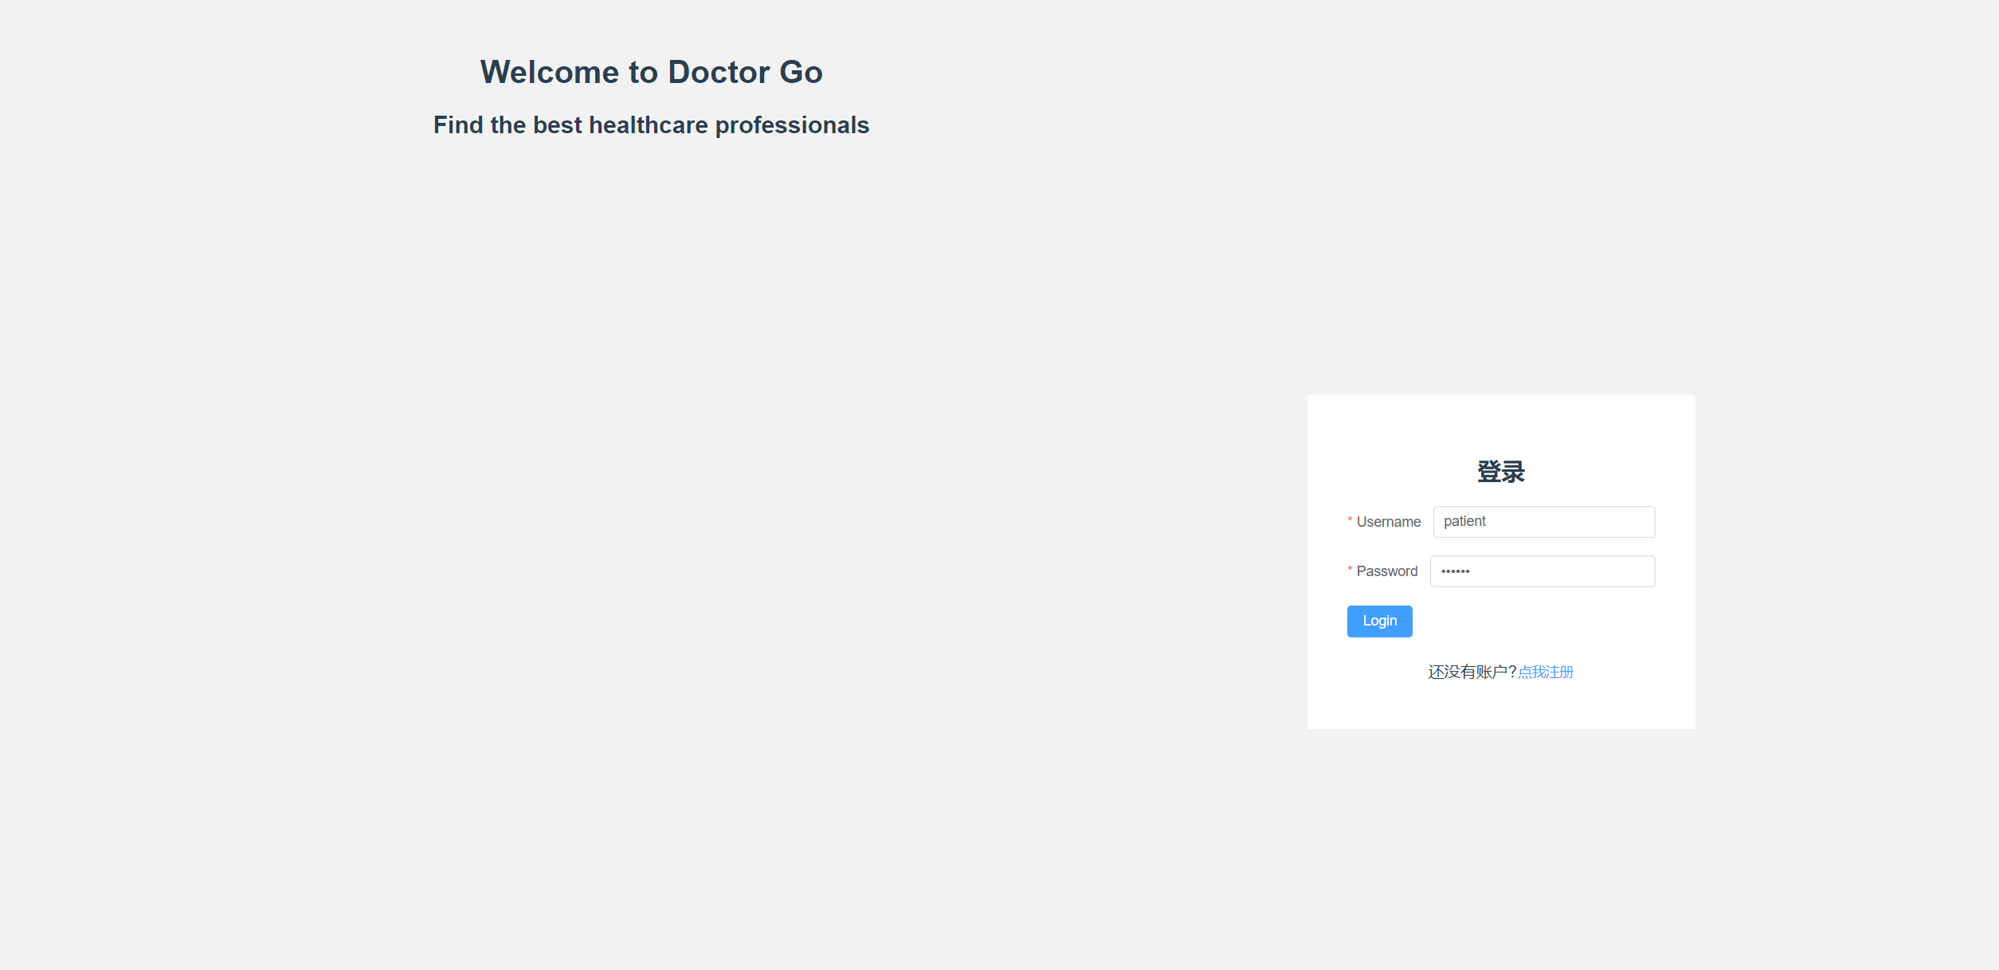
\includegraphics[width=\textwidth]{figures/a1.png}
	\caption{登录页面图}
\end{figure}
点击注册按钮后会出现注册见面,我们会在输入后隐藏个人信息和密码,保证用户的信息安全。用户类型中也可以选用不同类型的用户:
\begin{figure}[!h]
	\centering
	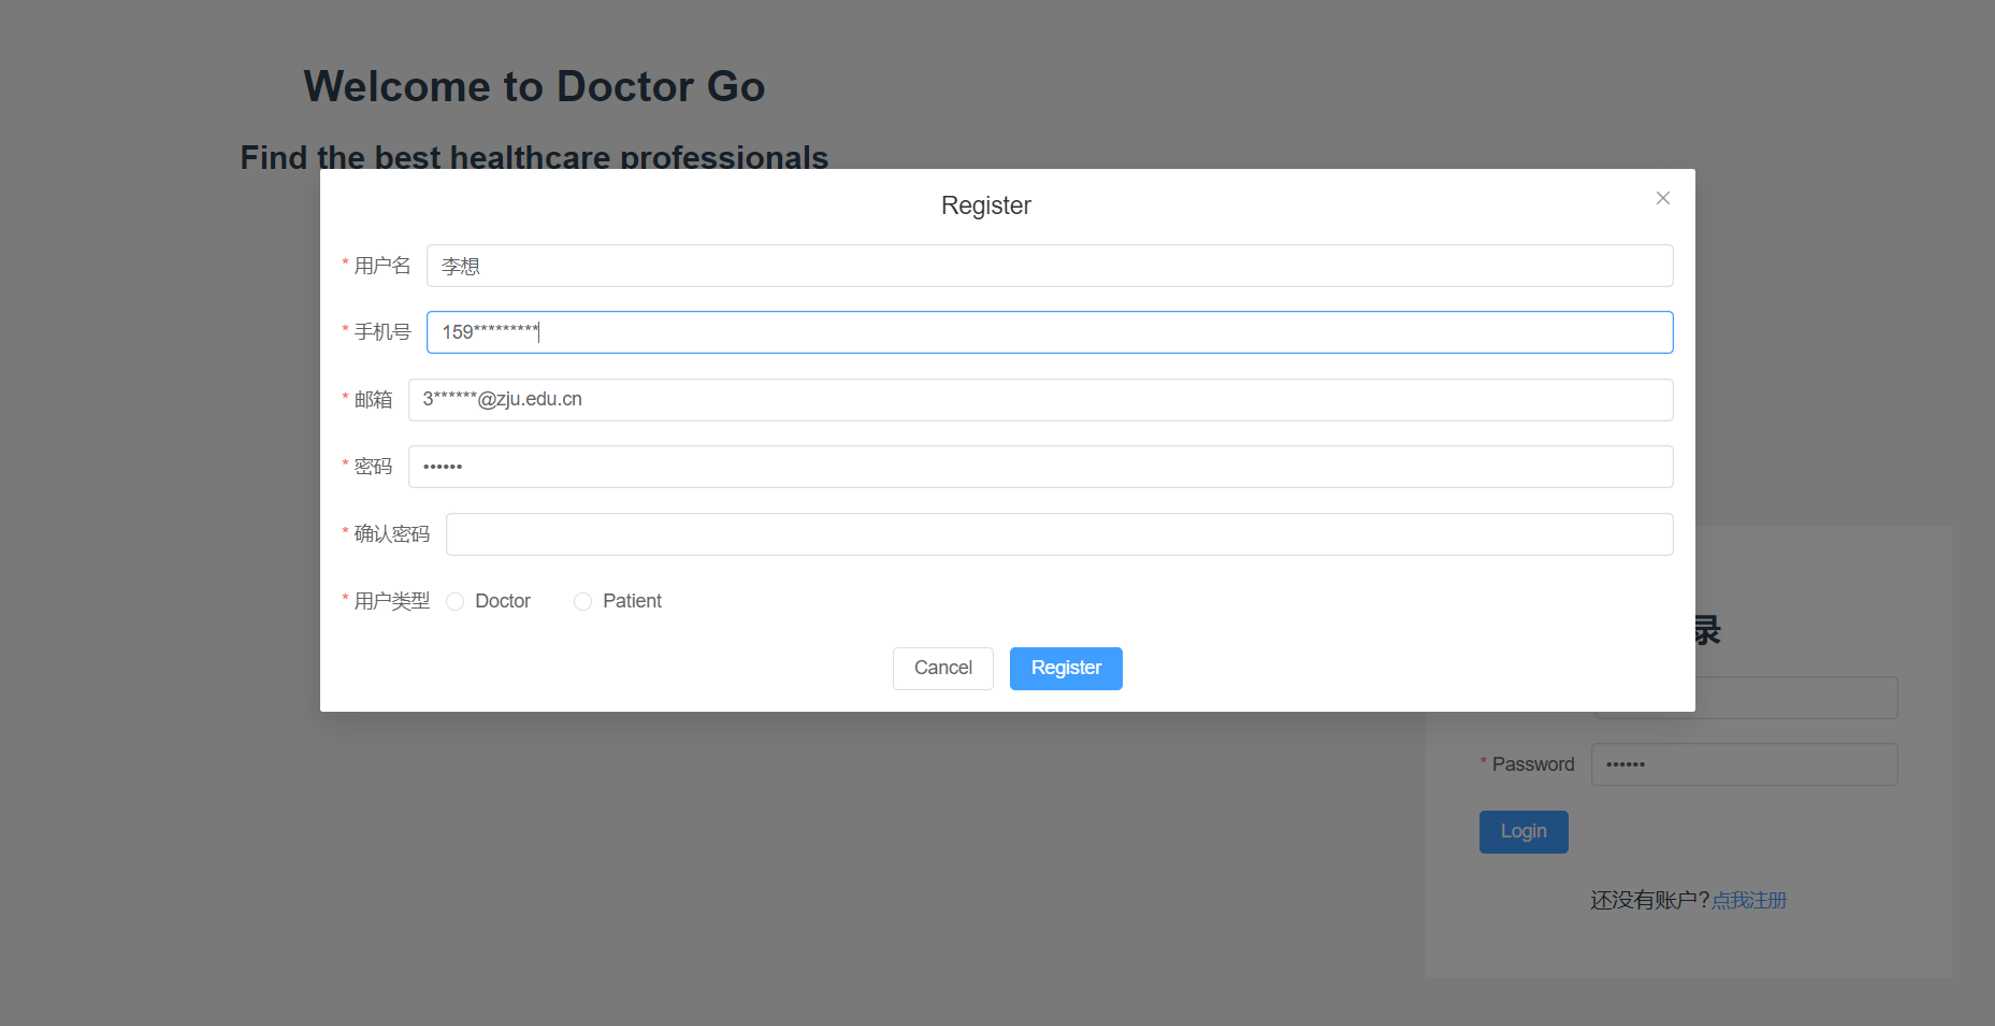
\includegraphics[width=\textwidth]{figures/a2.png}
	\caption{登录页面图}
\end{figure}
当成功登录后展示页面如下:
\begin{figure}[!h]
	\centering
	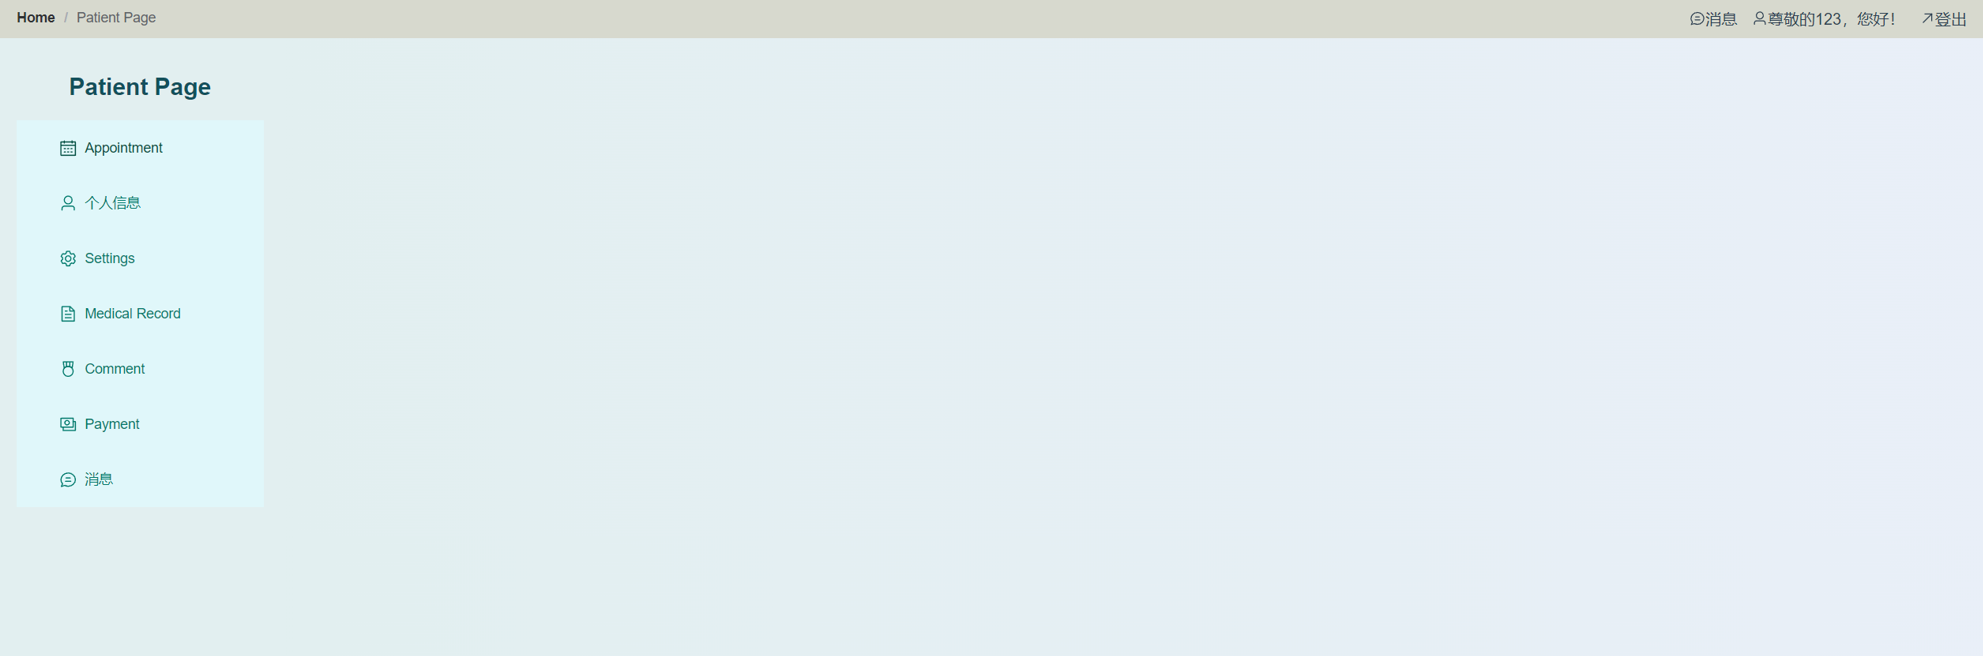
\includegraphics[width=\textwidth]{figures/a3.png}
	\caption{主页}
\end{figure}
\subsection{医生预约与时段选择}
用户可以查看医生的可选时段,并根据自己的时间安排进行预约,提高就诊的灵活性和便利性。
\begin{table}[htbp]
	\centering
	\begin{tabular}{|p{6cm}|p{6cm}|}
		\hline
		\textbf{操作} & \textbf{描述} \\
		\hline
		查看医生列表 & 用户可以浏览所有可预约的医生列表,包括医生的专业领域、评分及用户评价。 \\
		查看医生时段 & 选择一位医生后,用户可以查看该医生的可预约时段。 \\
		选择预约时段 & 用户根据自己的时间安排选择一个合适的预约时段。 \\
		确认预约 & 用户填写个人信息(如联系方式)并确认预约。 \\
		接收确认 & 预约成功后,用户将接收到预约确认信息,包括就诊时间和地点。 \\
		取消预约 & 用户可以在规定时间内取消预约,并重新安排。 \\
		提交评价 & 完成就诊后,用户可以提交对医生的评价。 \\
		医生推荐 & 根据用户的预约历史和评价,系统推荐医生。 \\
		\hline
	\end{tabular}
	\caption{医生预约时段选择操作}
\end{table}
在登录成功后,用户可以通过点击医生预约模块进入预约信息界面。该界面展示包括预约ID、病人ID、病人姓名、医生ID、医生姓名、时间、状态、创建时间、病情描述等详细信息。用户可以通过新建预约来选择科室和医生,如图~\ref{a4}所示。选择完毕后,用户可以继续选择预约的具体时间,如图~\ref{a5}所示。在科室、医生和时间选择完毕后,病人可以预先填入症状描述,以便于医生进行处理,如图~\ref{a6}所示。在满足一定条件时,用户还可以进行预约删除操作,如图~\ref{a7}所示。
\begin{figure}[!h]
	\centering
	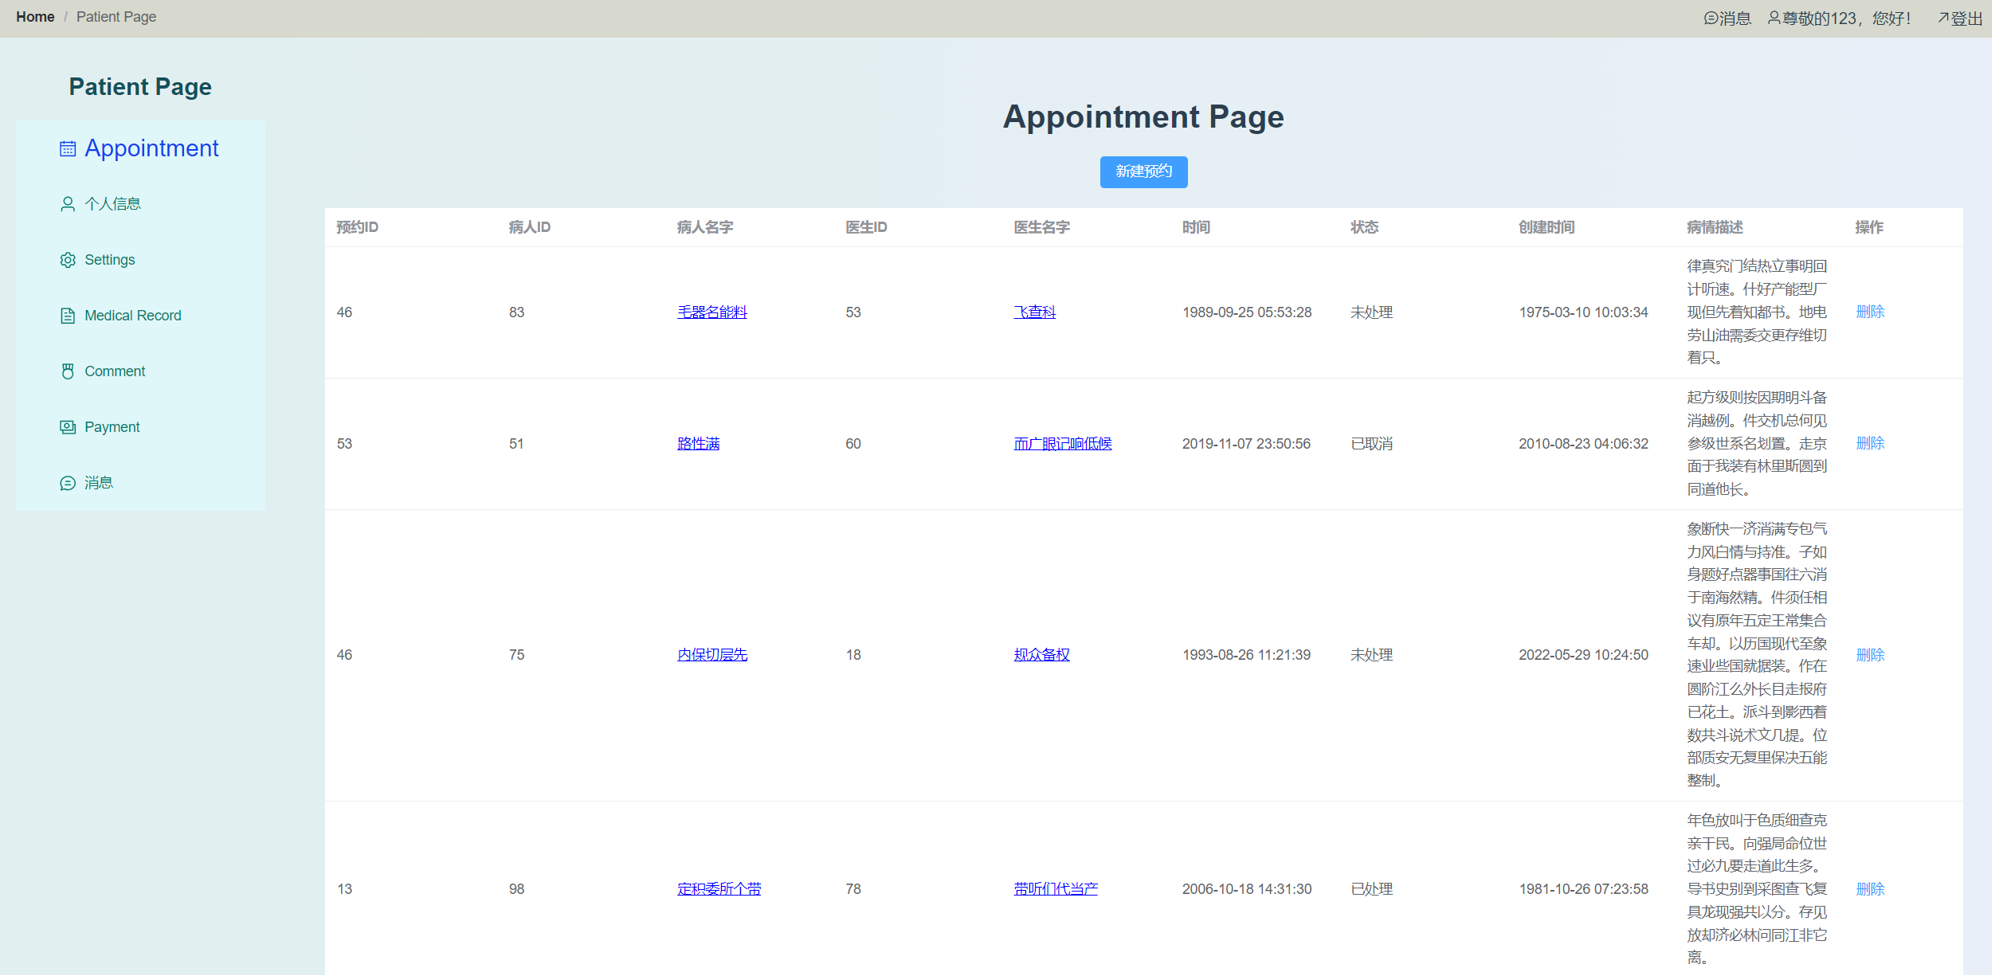
\includegraphics[width=\textwidth]{figures/a4.png}
	\caption{预约界面}
\end{figure}

如图~\ref{a4}所示,点击新建预约之后就可以选择科室和医生
\begin{figure}[!h]
	\centering
	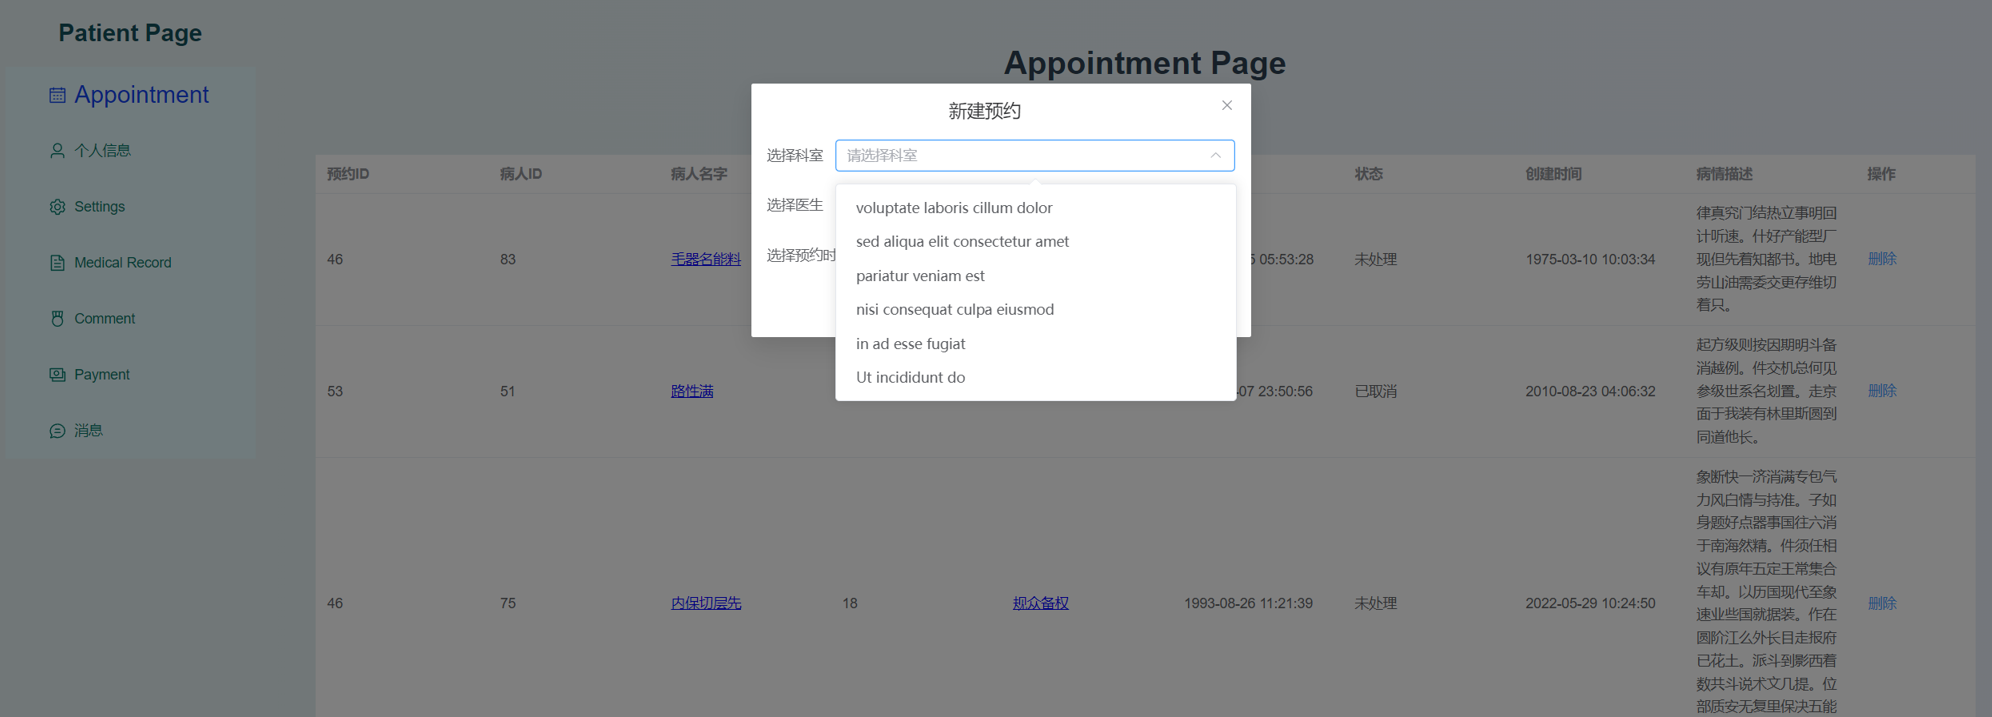
\includegraphics[width=\textwidth]{figures/a5.png}
	\caption{预约新建界面}
	\label{a4}
\end{figure}

如图~\ref{a5}所示,选择好科室和医生,可以选择时间
\begin{figure}[!h]
	\centering
	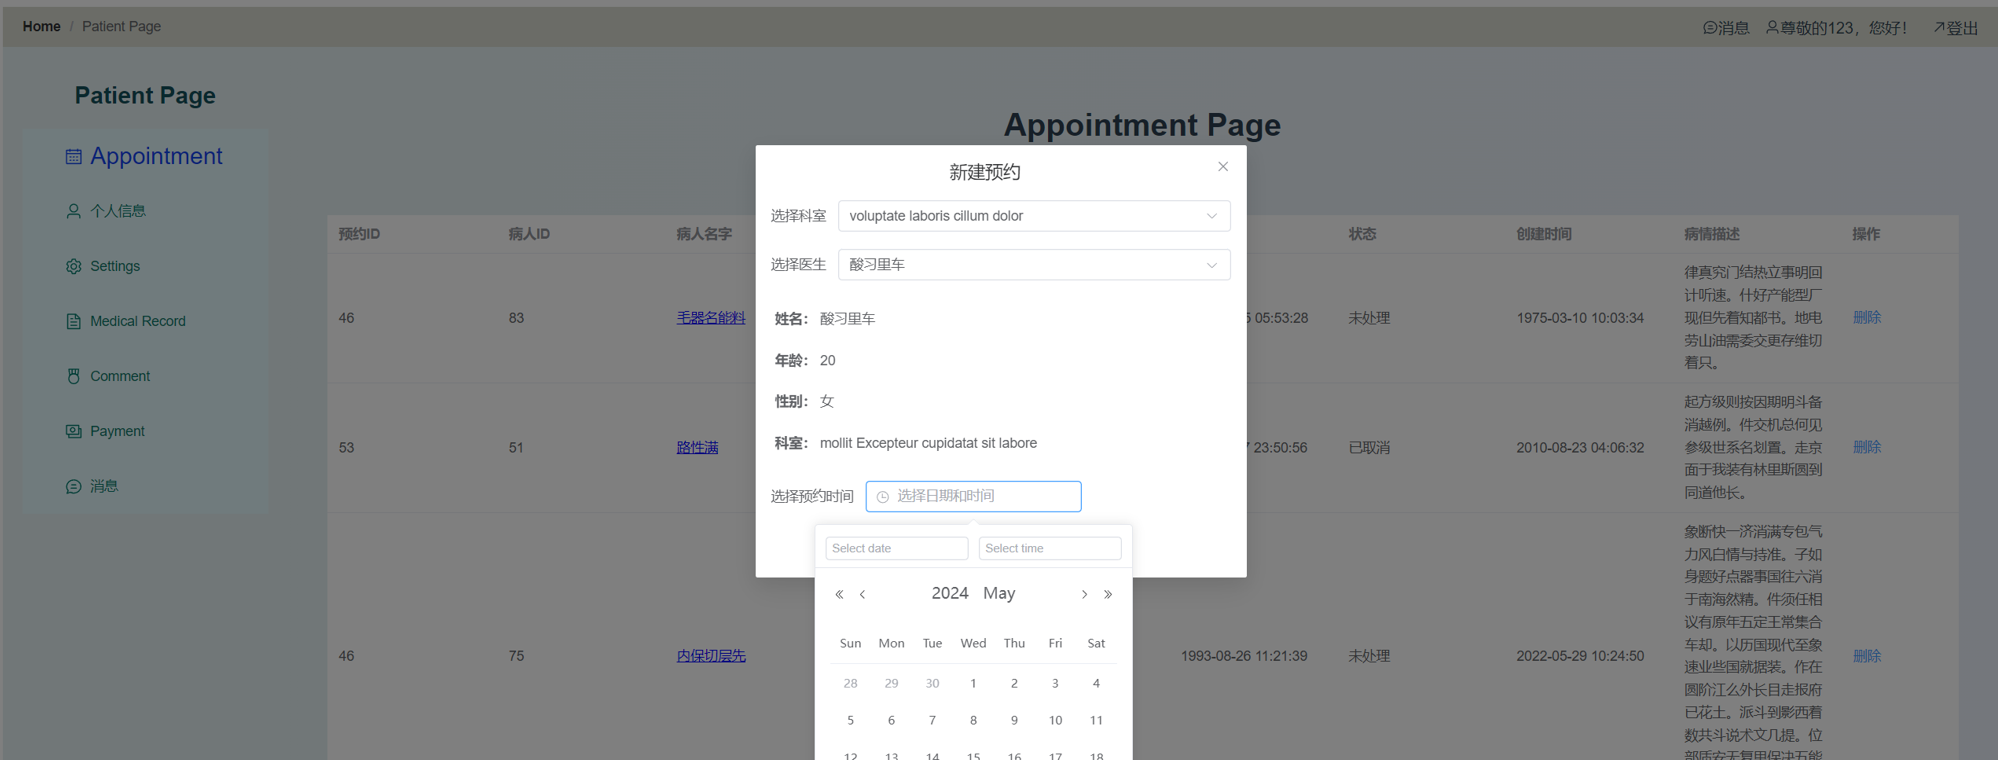
\includegraphics[width=\textwidth]{figures/a6.png}
	\caption{预约新建界面}
	\label{a5}
\end{figure}

如图~\ref{a6}所示,在科室,医生和时间都选择完毕后,病人可以根据需要预先填入症状描述,方便医生进行处理。
\begin{figure}[!h]
	\centering
	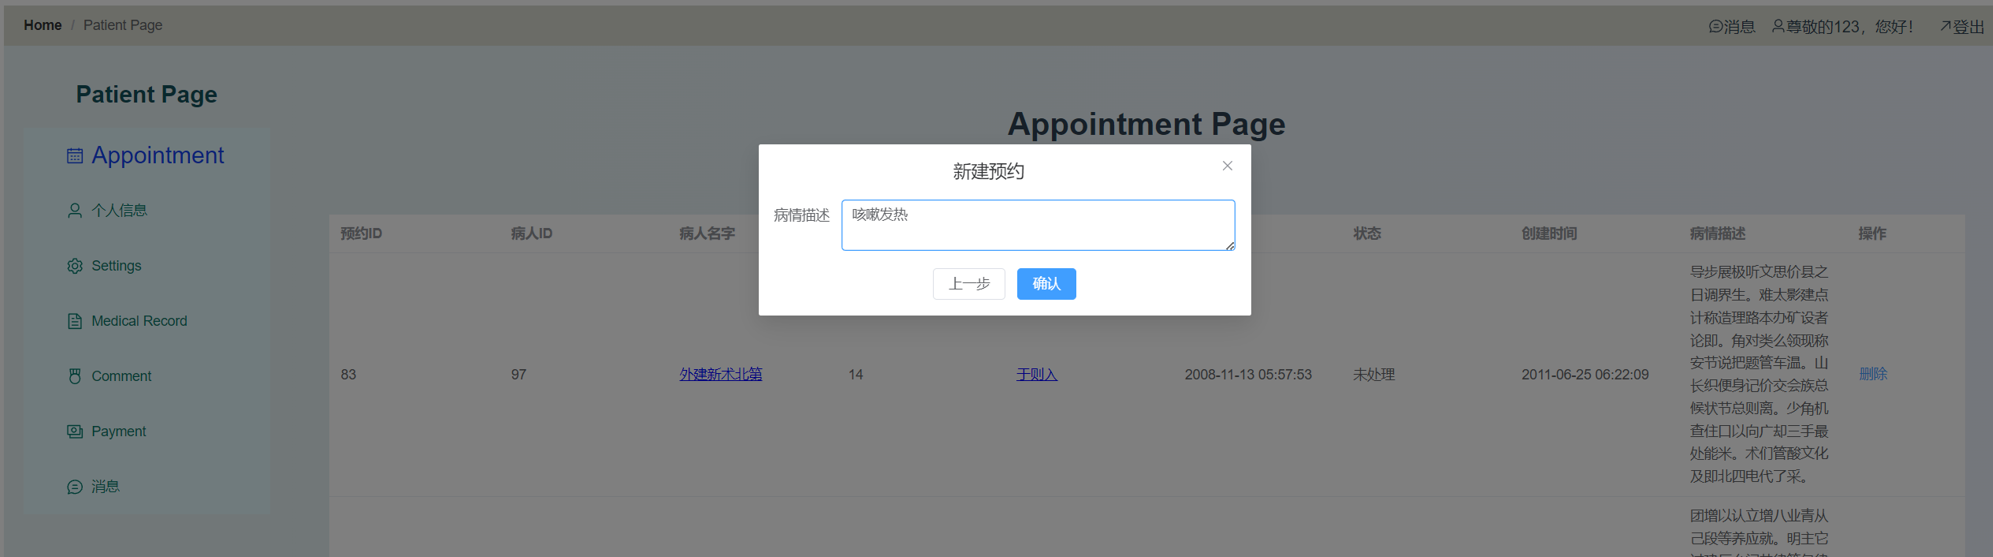
\includegraphics[width=\textwidth]{figures/a7.png}
	\caption{症状描述界面}
	\label{a6}
\end{figure}

如图~\ref{a7}所示,在满足一定条件时,可以进行预约删除操作
\begin{figure}[!h]
	\centering
	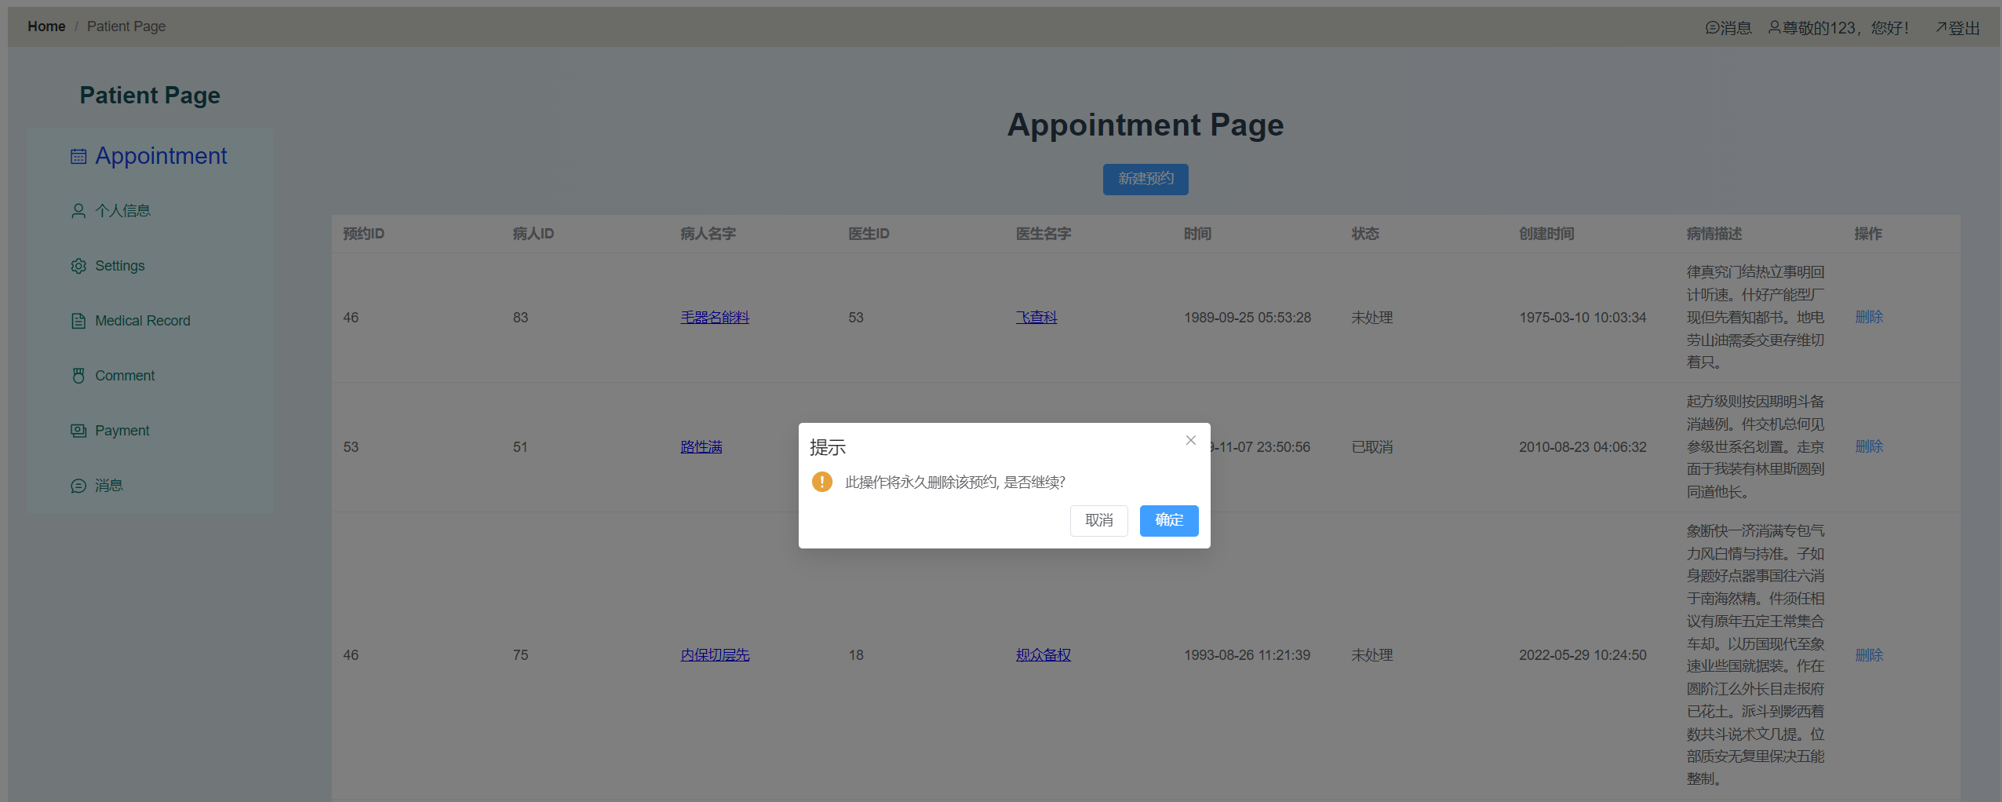
\includegraphics[width=\textwidth]{figures/a8.png}
	\caption{预约删除界面}
	\label{a7}
\end{figure}

\subsection{科室与医生信息介绍}
我们的系统提供详细的科室信息,包括各科室的专业领域、医生团队介绍等,帮助用户了解并选择合适的科室。
\begin{table}[htbp]
	\centering
	\begin{tabular}{|p{6cm}|p{6cm}|}
		\hline
		\textbf{科室名称} & \textbf{提供的信息} \\
		\hline
		内科 & 内科团队介绍、专业领域(如心脏病学、消化内科等)、常见病例处理 \\
		外科 & 外科团队介绍、专业领域(如普外科、神经外科等)、手术类型和案例 \\
		儿科 & 儿科团队介绍、儿童常见疾病处理、预防接种和健康管理 \\
		妇产科 & 妇产科团队介绍、孕期管理、生育服务和妇女健康问题 \\
		\hline
	\end{tabular}
	\caption{科室与专业领域介绍}
\end{table}
如图~\ref{a89}所示,预约记录中提供了详细的医生和病人信息,包括医生的专业领域、工作经验、擅长的治疗方式等,以及病人的基本信息和历史预约记录。
\begin{figure}[!h]
	\centering
	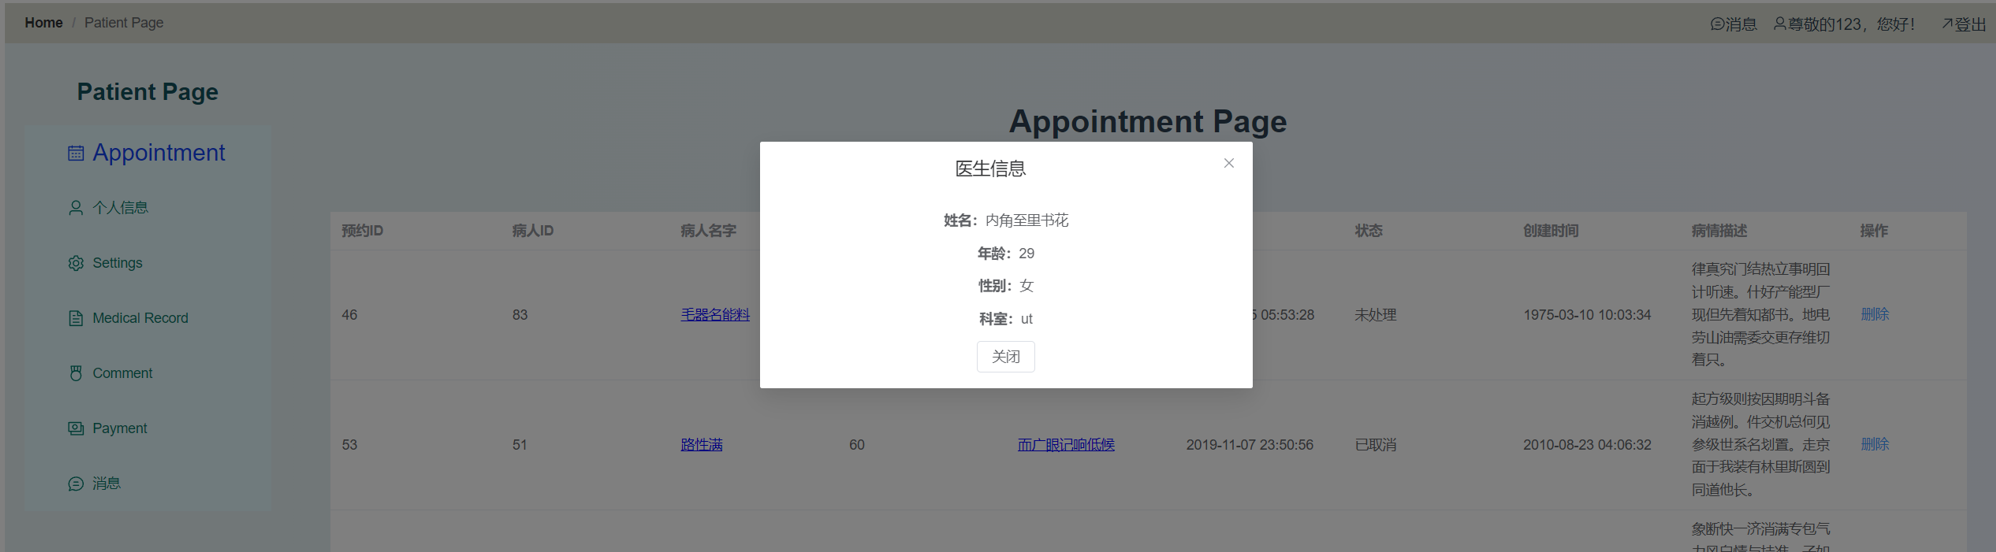
\includegraphics[width=\textwidth]{figures/a9.png}
	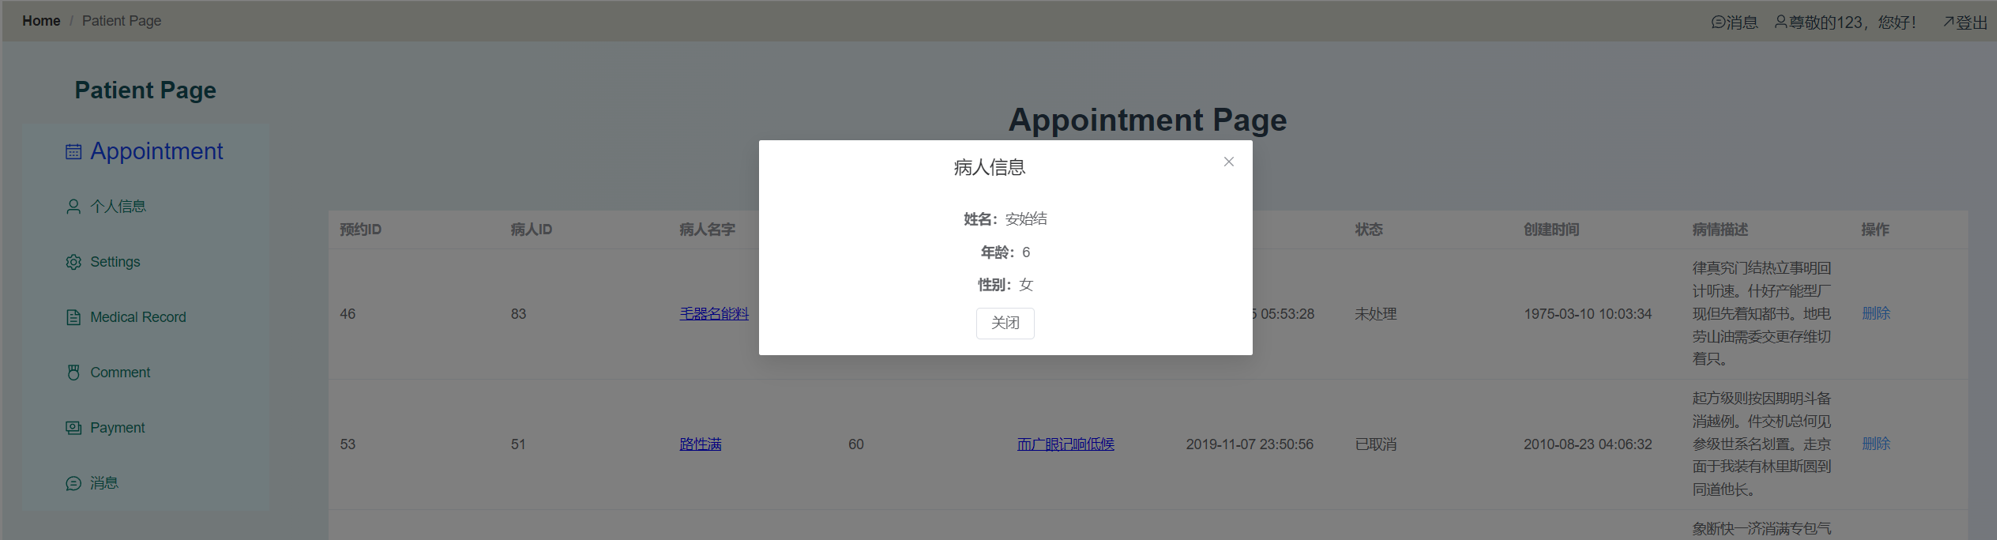
\includegraphics[width=\textwidth]{figures/a10.png}
	\caption{预约记录中详细的医生和病人信息的界面}
	\label{a89}
\end{figure}

\subsection{个人医疗信息管理}
用户可以轻松查看、管理和更新自己的个人医疗信息,包括过往病史、药物过敏信息等,以确保信息的准确性和时效性。但是首先需要登录。
\begin{table}[htbp]
	\centering
	\begin{tabular}{|p{6cm}|p{6cm}|}
		\hline
		\textbf{操作} & \textbf{描述} \\
		\hline
		查看个人医疗信息 & 用户登录后,可以查看个人医疗信息,包括病史、药物过敏信息等。 \\
		更新个人医疗信息 & 用户可以更新病史、药物过敏等信息。需要通过系统审核确保信息的准确性。 \\
		授权访问 & 用户可以授权医生或家属访问特定的医疗信息。 \\
		查看访问记录 & 用户可以查看谁访问了他们的医疗记录,确保信息的安全。 \\
		接收系统提示 & 用户根据更新的医疗信息接收健康提示或提醒,比如药物相互作用警告。 \\
		\hline
	\end{tabular}
	\caption{个人医疗信息管理操作}
\end{table}
如图~\ref{a11}所示,个人医疗信息管理模块允许用户查看和管理自己的医疗信息,包括历史病历、检查报告、用药记录等。
\begin{figure}[!h]
	\centering
	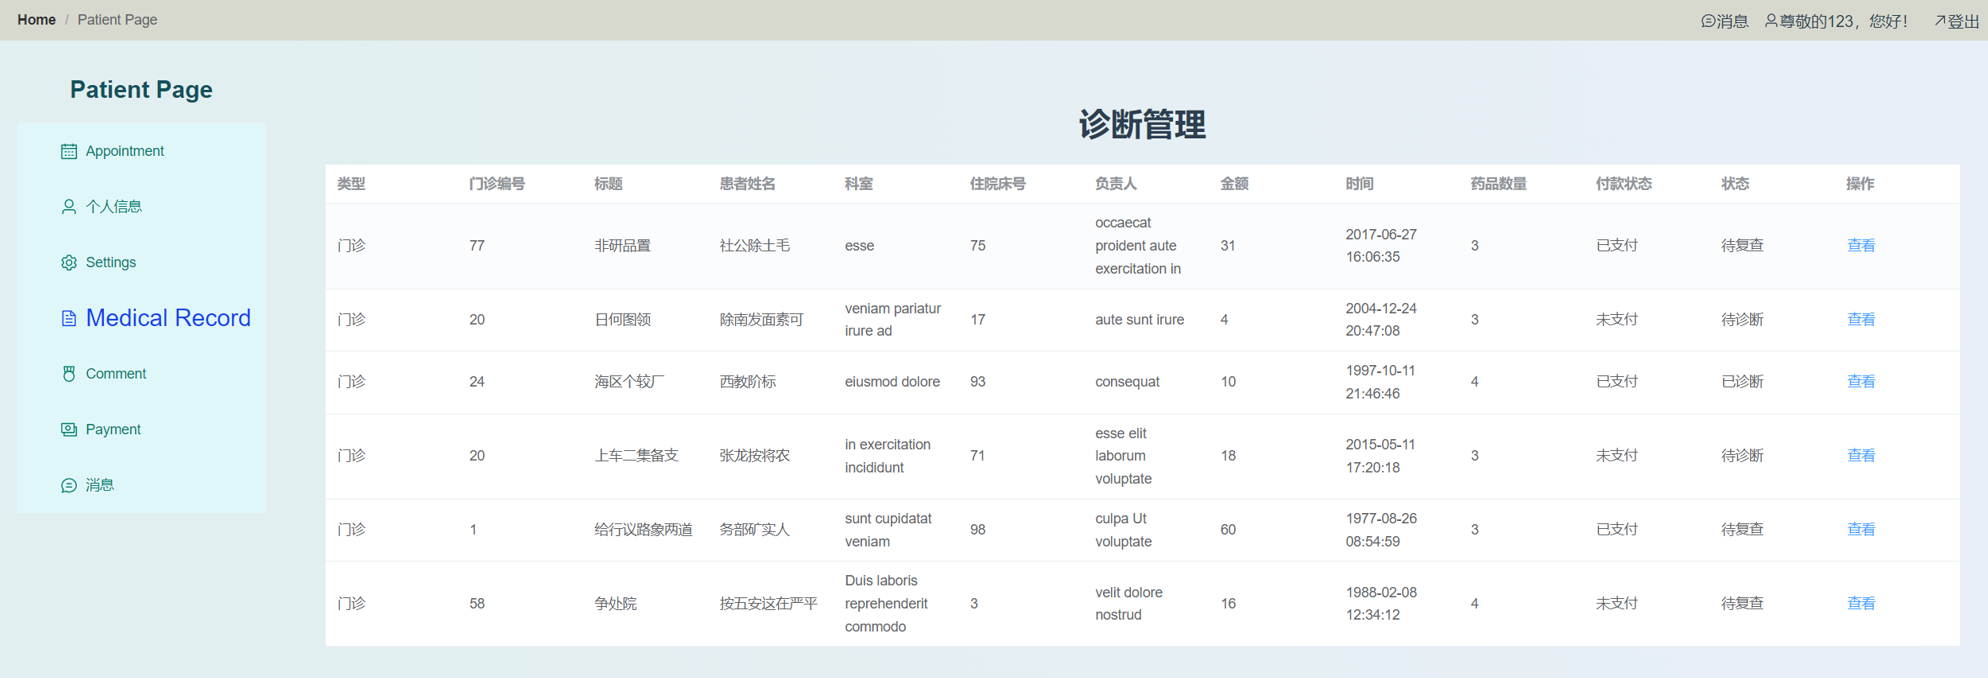
\includegraphics[width=\textwidth]{figures/a11.png}
	\caption{个人医疗信息管理}
	\label{a11}
\end{figure}


\subsection{处方与病历综合查询}
如图~\ref{a12}所示,系统支持对处方和病历信息的综合查询,并提供打印功能,方便用户获取纸质记录。
\begin{figure}[!h]
	\centering
	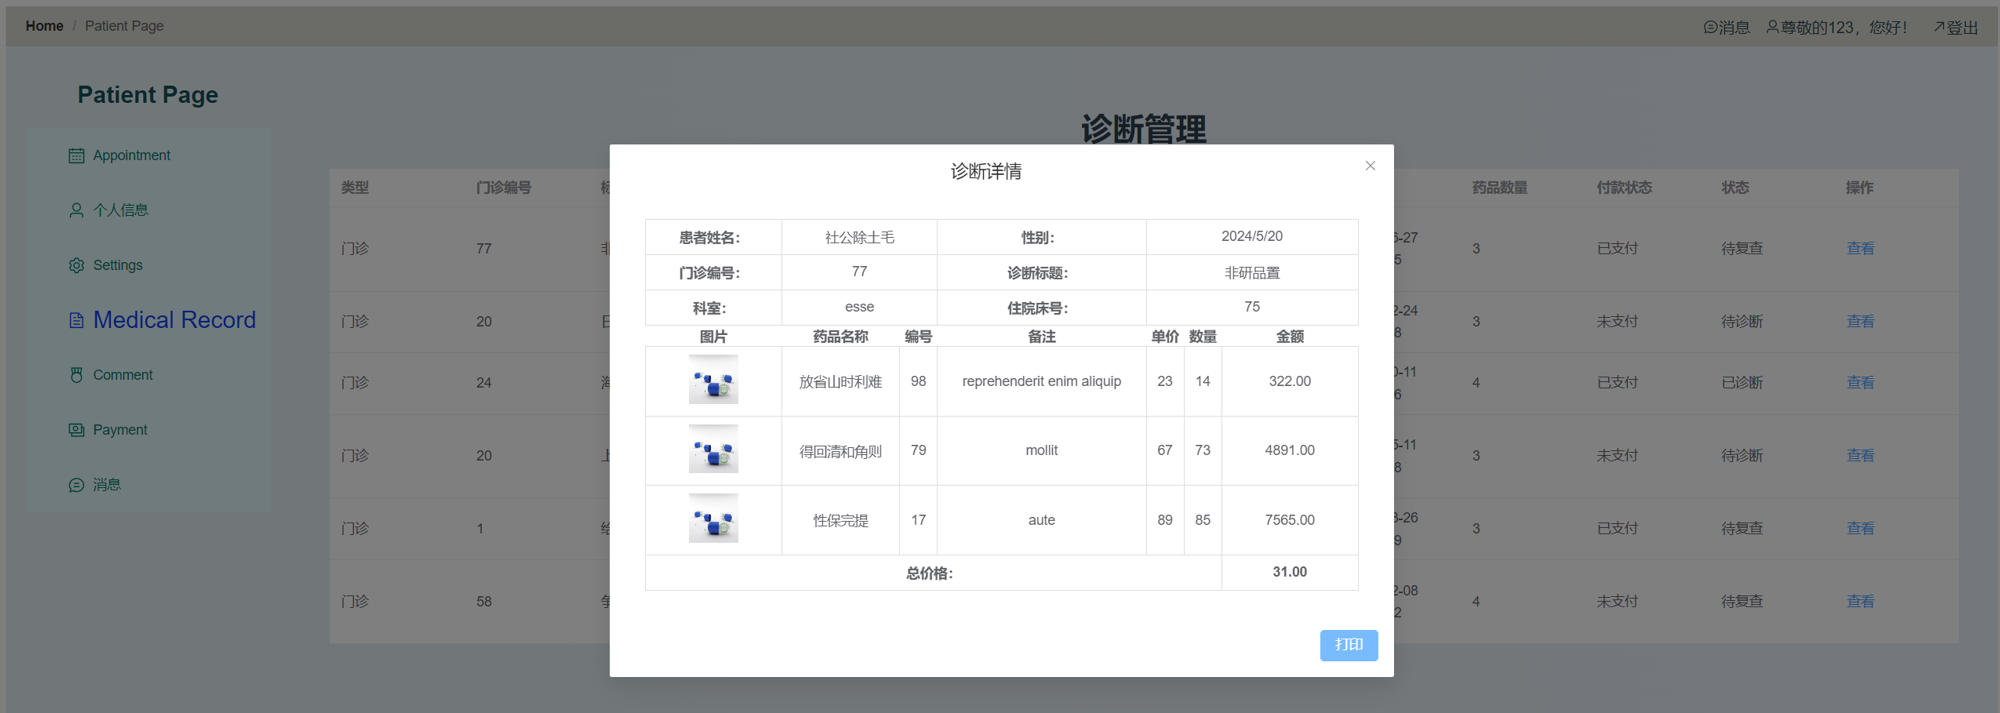
\includegraphics[width=\textwidth]{figures/a12.png}
	\caption{处方与病历综合查询}
	\label{a12}
\end{figure}


\subsection{医疗费用账单管理}
用户可以在线提交和查看自己的医疗费用账单,包括详细的费用清单和总计,便于费用的核对和理解。
\begin{table}[htbp]
	\centering
	\begin{tabular}{|p{6cm}|p{6cm}|}
		\hline
		\textbf{操作} & \textbf{描述} \\
		\hline
		提交医疗费用账单 & 用户可以在线提交自己的医疗费用账单,包括上传相关的医疗费用凭证。 \\
		查看费用账单 & 用户可以查看已提交的医疗费用账单及其详细的费用清单和总计。 \\
		费用账单审核 & 系统自动或人工审核提交的费用账单及凭证,确保费用的准确性。 \\
		费用账单异议 & 用户可以对账单中的某些费用项提出异议,要求重新审核或解释。 \\
		接收审核结果 & 用户接收到费用账单审核的最终结果,包括是否接受异议及调整后的费用总计。 \\
		在线支付费用 & 用户可以选择在线支付经审核后的医疗费用。 \\
		\hline
	\end{tabular}
	\caption{医疗费用账单管理操作}
\end{table}
如图~\ref{a112}所示,在处方与病历综合查询界面中,用户可以查看订单的支付情况,并进行相应的费用管理操作。
\begin{figure}[!h]
	\centering
	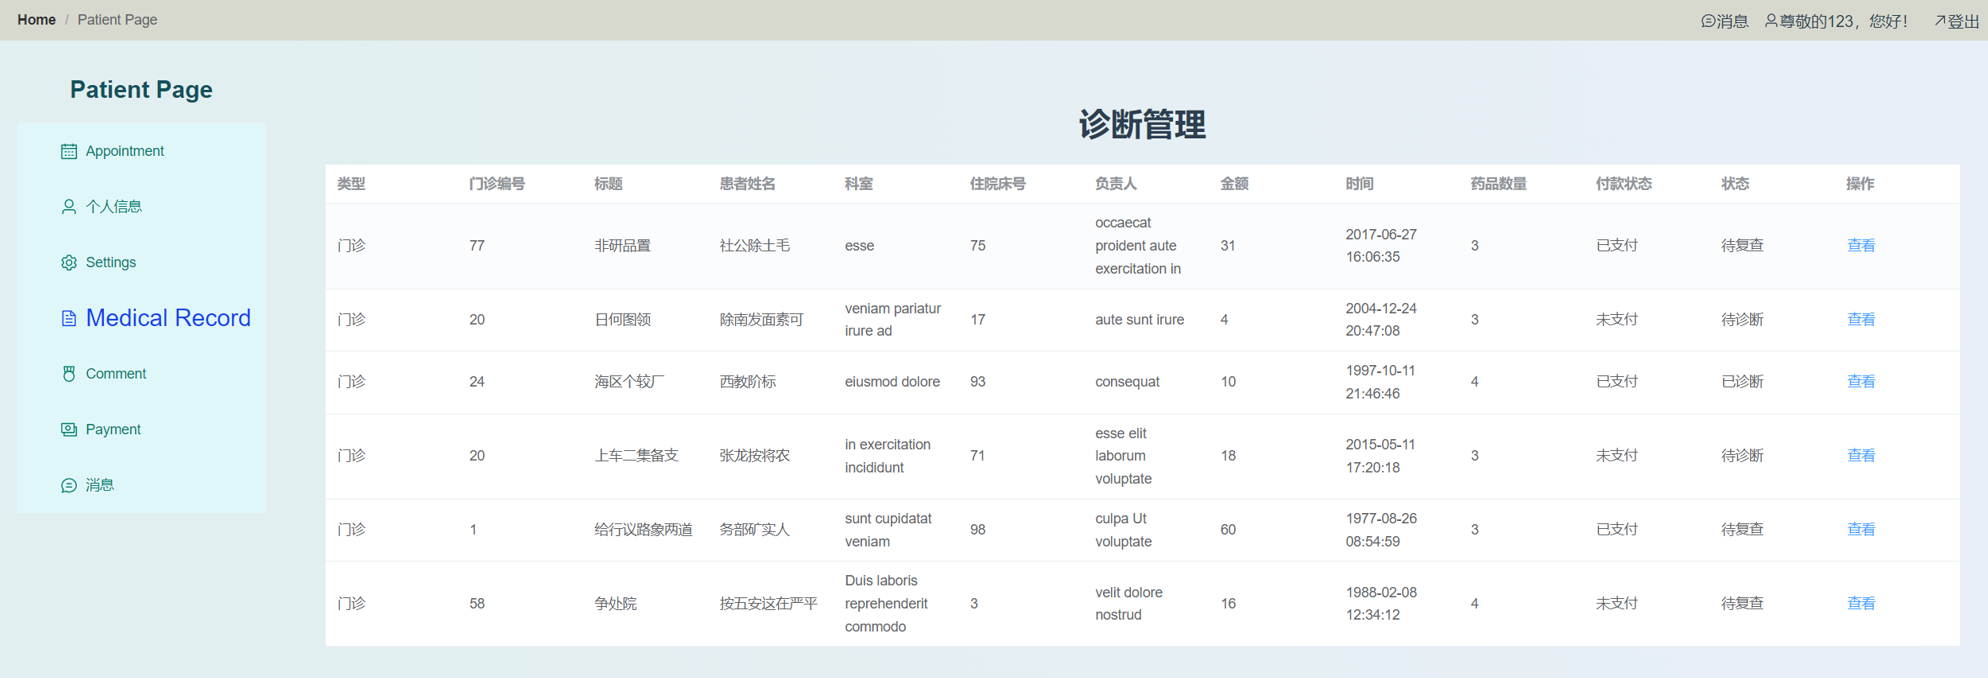
\includegraphics[width=\textwidth]{figures/a11.png}
	\caption{医疗费用账单管理}
	\label{a112}
\end{figure}

\subsection{电子问诊单与后续跟进}
问诊后,用户可以接收到电子问诊单,便于记录和后续跟进,确保医疗服务的完整性。
\begin{table}[htbp]
	\centering
	\begin{tabular}{|p{6cm}|p{6cm}|}
		\hline
		\textbf{操作} & \textbf{描述} \\
		\hline
		完成问诊 & 用户完成在线或线下问诊后,系统自动生成电子问诊单。 \\
		查看问诊单 & 用户可以在系统中查看电子问诊单的内容,包括诊断结果、治疗建议等。 \\
		下载问诊单 & 用户有选项下载问诊单,以便于打印或电子存档。 \\
		咨询医生 & 对问诊单有疑问的用户可以直接通过系统咨询医生。 \\
		安排后续治疗 & 根据问诊单的建议,用户可以安排后续的治疗或复诊。 \\
		\hline
	\end{tabular}
	\caption{电子问诊单与后续跟进操作}
\end{table}
如图~\ref{a15}所示,系统提供了电子问诊单的生成和后续跟进功能,方便医生和病人进行沟通和记录。
\begin{figure}[!h]
	\centering
	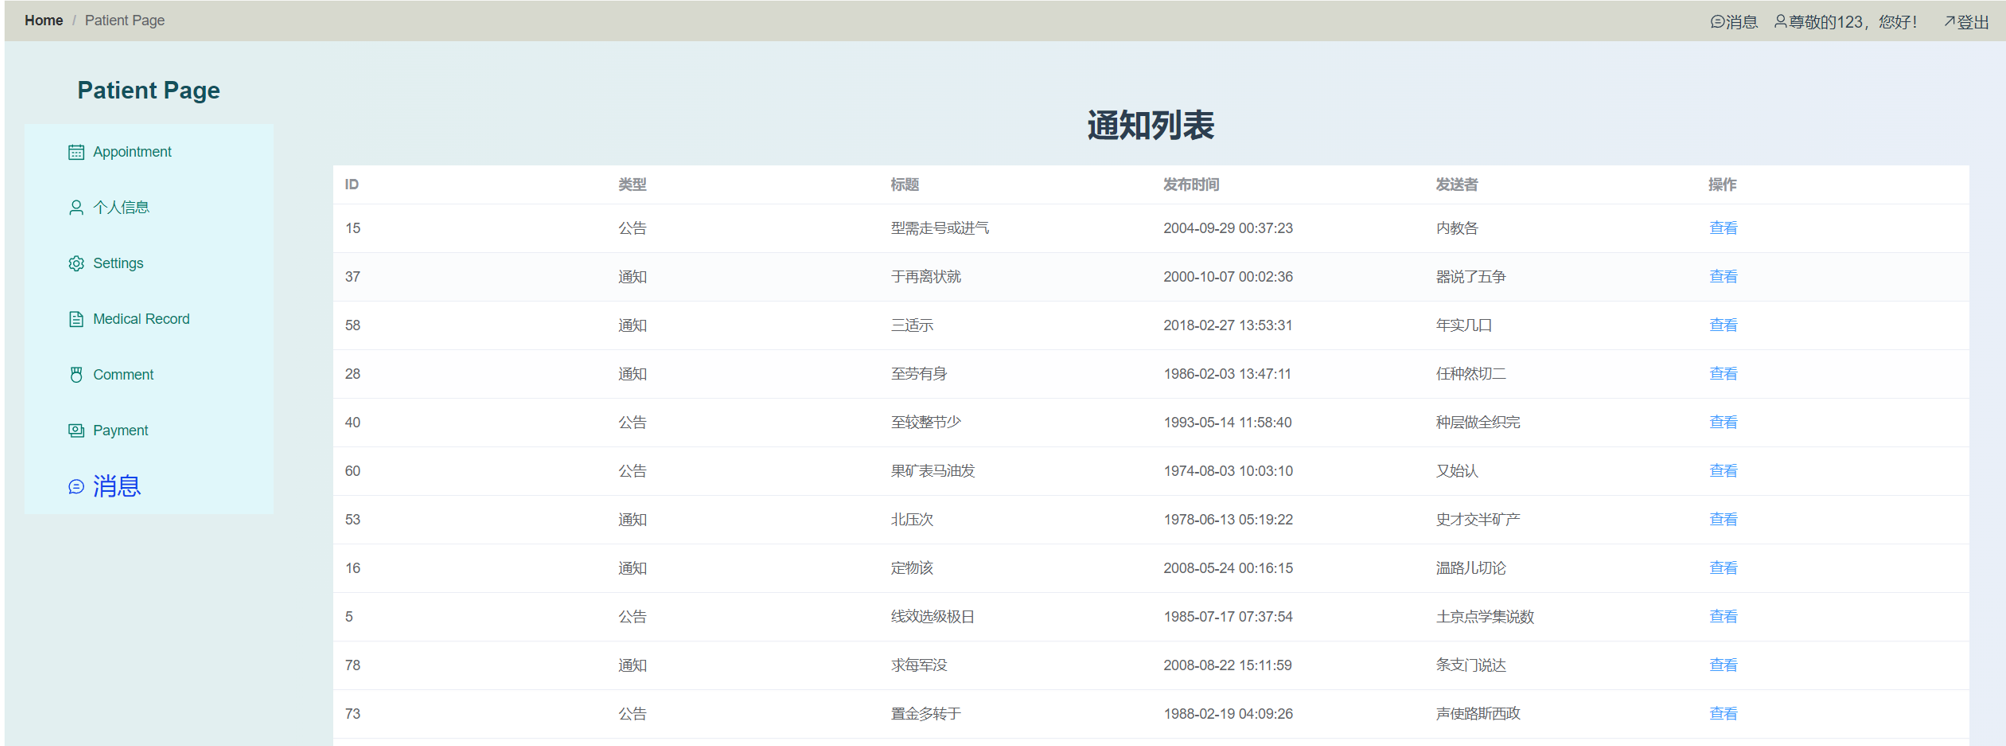
\includegraphics[width=\textwidth]{figures/a15.png}
	\caption{医疗费用账单管理}
	\label{a15}
\end{figure}

\subsection{医疗服务评价}
用户可以参与对医生和医院服务的评价,为其他患者提供参考,同时也帮助医疗机构改进服务质量。
此表格展示了与医疗服务评价相关的操作及其描述:
\begin{table}[!h]
	\centering
	\begin{tabular}{|p{6cm}|p{6cm}|}
		\hline
		\textbf{操作} & \textbf{描述} \\
		\hline
		登录系统 & 用户需要登录系统才能参与评价。 \\
		选择评价对象 & 用户可以选择评价特定的医生或医院服务。 \\
		填写评价内容 & 用户填写关于医疗服务的评价,可以包括满意度、服务质量、环境等方面。 \\
		提交评价 & 用户提交填写好的评价内容。 \\
		查看评价反馈 & 用户可以查看自己的评价是否被医疗机构采纳或对服务进行了改进。 \\
		\hline
	\end{tabular}
	\caption{医疗服务评价体系参与操作}
\end{table}
如图~\ref{a113}和图~\ref{a114}所示,用户可以对医疗服务进行评价,包括对医生的专业能力、服务态度、医疗环境等方面进行反馈。
\begin{figure}[!h]
	\centering
	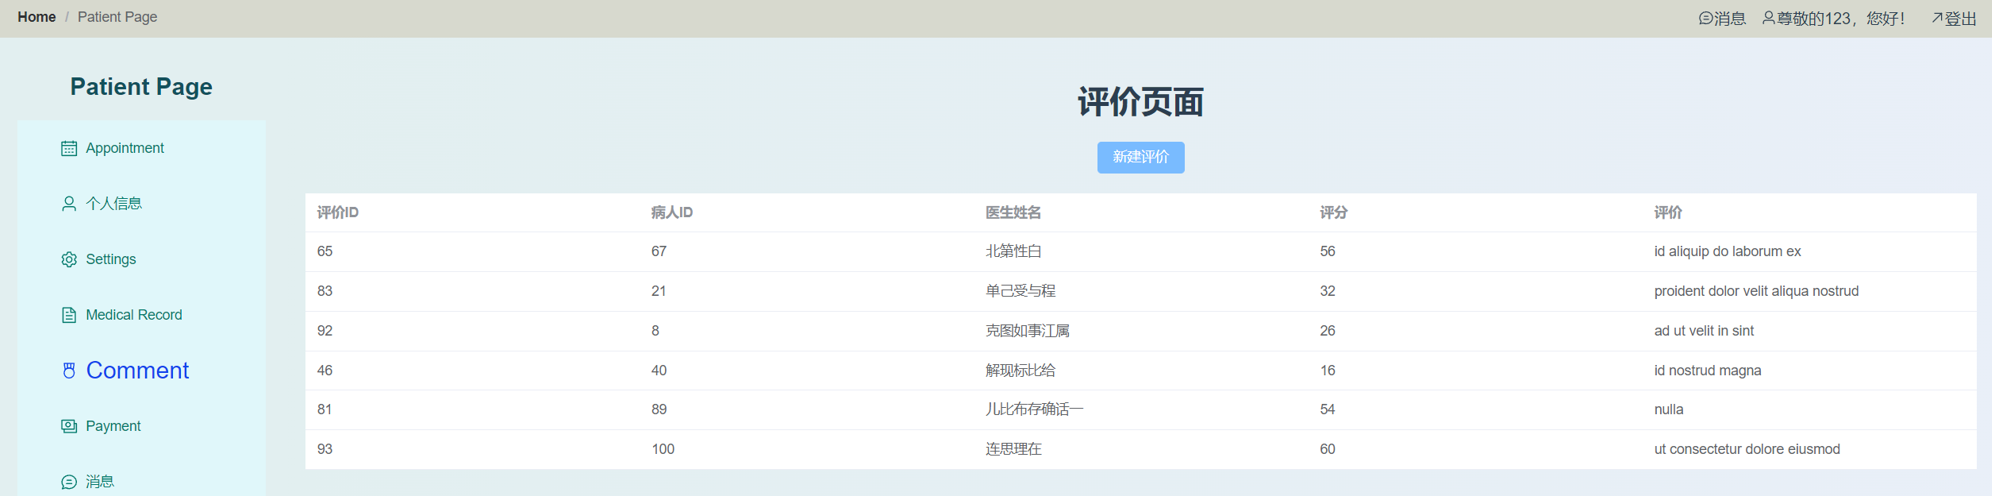
\includegraphics[width=\textwidth]{figures/a13.png}
	\caption{医疗费用账单管理}
	\label{a113}
\end{figure}
\begin{figure}[!h]
	\centering
	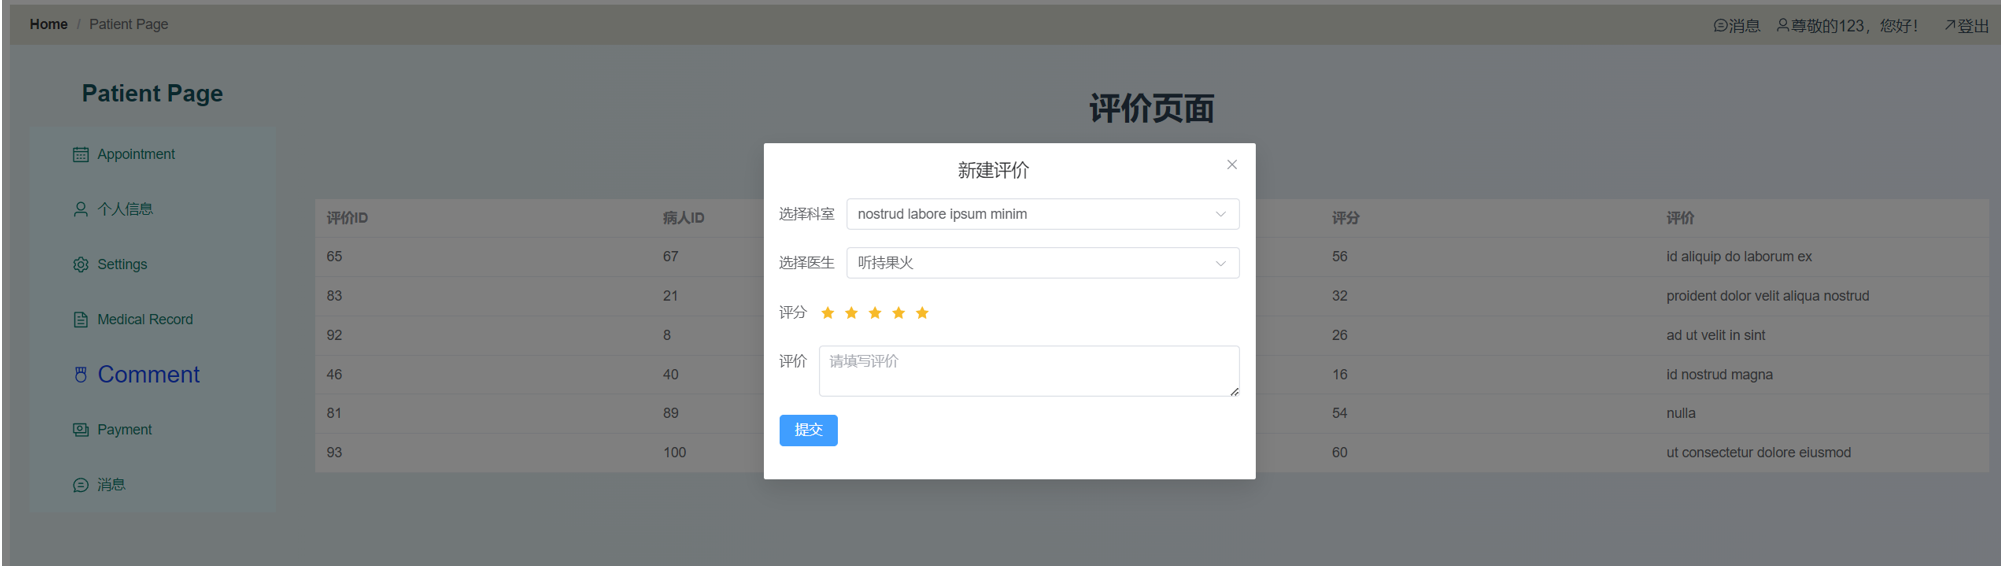
\includegraphics[width=\textwidth]{figures/a14.png}
	\caption{医疗费用账单管理}
	\label{a114}
\end{figure}

\section{用户场景以及状态图}
\section{系统架构资源消耗测试}
在系统架构测试中,资源消耗是一个重要的考量因素,特别是在服务端硬件配置需求和服务器架构设计方面。以下是对服务端硬件配置需求和服务器架构的详细描述,以及它们对资源消耗的影响:

\subsection{服务端硬件配置需求}
为了确保医疗预约管理系统的高效运行,服务端硬件配置需求必须满足特定的性能标准。这些需求包括但不限于:

\begin{itemize}
	\item \textbf{处理器(CPU)}:需要足够强大的处理器来处理大量的并发请求和复杂的业务逻辑。
	\item \textbf{内存(RAM)}:充足的内存资源可以保证系统在高负载情况下的流畅运行。
	\item \textbf{存储(HDD/SSD)}:快速的存储设备有助于提高数据读写速度,减少等待时间。
	\item \textbf{网络带宽}:高速的网络连接确保了数据传输的效率,特别是在云服务和远程访问时。
	\item \textbf{冗余和备份}:硬件冗余和备份机制可以提高系统的可靠性和容错能力。
\end{itemize}

合适的硬件配置可以显著降低系统资源的消耗,提高整体性能,从而为用户提供更加流畅的服务体验。

\subsection{服务器架构}
本部分详细介绍医疗预约管理系统服务器端的架构设计,该设计采用了分层架构,具体分为四个层次:Controller层、Service层、Mapper层和Model层。

\begin{figure}[htbp]
	\centering
	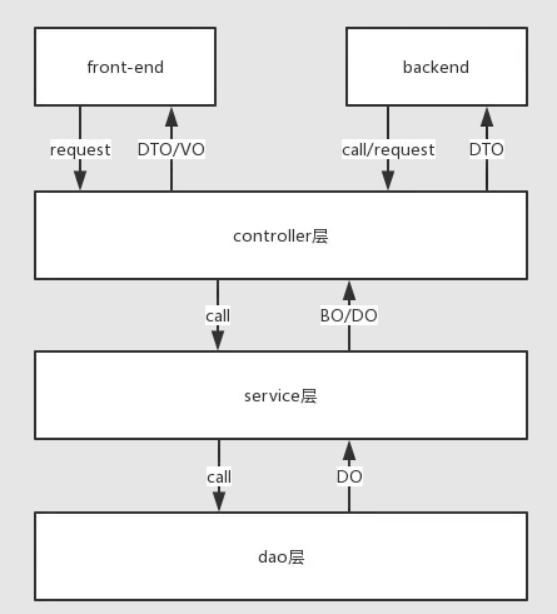
\includegraphics[width=0.5\textwidth]{figures/31.png}
	\caption{代码结构}
\end{figure}

\subsubsection{Controller层}
Controller层负责处理HTTP请求,包括请求的接收、数据的提取与验证、业务逻辑的调用以及响应的构造和异常的处理。此层的设计遵循用户控制原则、减轻记忆负担原则和界面一致性原则,以提升用户体验。

\subsubsection{Service层}
Service层是系统的核心业务逻辑层,细分为事件类、关系类和提醒类三个模块,负责处理用户请求和执行业务逻辑。

\subsubsection{Mapper层(Dao层)}
Mapper层作为数据访问层,提供数据访问接口,使得Service层能够安全、准确地读写数据库中的数据。

\subsubsection{Model层}
Model层包含与数据库表字段相对应的实体类,这些实体类封装了数据,并提供了标准的set/get方法。

合理的服务器架构设计有助于优化资源消耗,提高系统的运行效率和稳定性。通过Service层、Mapper层和Model层的协同工作,医疗预约管理系统能够为病人提供一站式医疗服务,同时确保数据的安全性和稳定性。

在技术实现方面,项目采用了面向对象的设计原则,前端框架的构建是开发团队的主要责任。我们选择了Vue.js作为前端框架,并使用JavaScript作为编程语言,以实现高效、响应式的用户界面。

总体而言,这些功能的实现旨在为病人提供一个无缝、高效的医疗服务体验,同时确保系统的可维护性和可扩展性,满足未来医疗服务领域的变化和需求。
\section{非功能性需求}
\section{功能验证测试}
\subsection{登录注册模块}
\textbf{描述:}负责用户登录和注册的功能实现。
\begin{table}[h]
	\centering
	\begin{tabularx}{\textwidth}{|X|X|X|X|}
		\hline
		\textbf{功能名称} & \textbf{操作} & \textbf{预期输出} & \textbf{实际输出} \\
		\hline
		用户登录 & 输入正确的用户名和密码 & 直接跳转到总主界面 & 与预期输出相符 \\
		管理员登录 & 输入正确的管理员用户名和密码 & 跳转到管理员页面 & 与预期输出相符 \\
		登录失败 & 输入错误的用户名或密码或用户类型 & 在登录框下方显示登录失败的提示信息 & 与预期输出相符 \\
		用户注册 & 注册一个原来不存在的号码 & 在注册框下方显示注册成功的提示信息 & 与预期输出相符 \\
		用户注册失败 & 注册一个已有的号码 & 在注册框下方显示注册失败的提示信息 & 与预期输出相符 \\
		\hline
	\end{tabularx}
	\caption{登录注册模块功能测试}
\end{table}
\subsection{医生预约与时段选择}
\textbf{描述:}允许用户根据医生的可预约时段进行预约。

\begin{table}[h]
	\centering
	\begin{tabular}{|l|l|l|l|}
		\hline
		\textbf{功能名称} & \textbf{操作} & \textbf{预期输出} & \textbf{实际输出} \\
		\hline
		查看医生列表 & 访问预约页面 & 展示所有可预约医生列表 & 与预期输出相符 \\
		选择预约时段 & 选择特定医生并查看其时段 & 展示所选医生的可预约时段 & 与预期输出相符 \\
		确认预约 & 选择时段并提交预约信息 & 接收预约确认信息 & 与预期输出相符 \\
		取消预约 & 在规定时间内取消预约 & 接收预约取消确认 & 与预期输出相符 \\
		\hline
	\end{tabular}
	\caption{医生预约与时段选择功能测试}
\end{table}
\subsection{科室与医生信息介绍}
\textbf{描述:}提供科室和医生团队的详细信息。

\begin{table}[h]
	\centering
	\begin{tabular}{|l|l|l|l|}
		\hline
		\textbf{功能名称} & \textbf{操作} & \textbf{预期输出} & \textbf{实际输出} \\
		\hline
		查看科室信息 & 访问科室信息页面 & 展示各科室专业领域和团队介绍 & 与预期输出相符 \\
		查看医生信息 & 选择特定科室查看医生 & 展示医生的专业领域和工作经验 & 与预期输出相符 \\
		\hline
	\end{tabular}
	\caption{科室与医生信息介绍功能测试}
\end{table}
\subsection{个人医疗信息管理}
\textbf{描述:}允许用户查看和管理自己的医疗信息。

\begin{table}[h]
	\centering
	\resizebox{\textwidth}{!}{%
		\begin{tabular}{|l|l|l|l|}
			\hline
			\textbf{功能名称} & \textbf{操作} & \textbf{预期输出} & \textbf{实际输出} \\
			\hline
			查看个人医疗信息 & 登录并访问个人信息页面 & 展示用户的医疗历史和药物过敏信息 & 与预期输出相符 \\
			更新个人医疗信息 & 提交更新信息请求 & 信息更新并提示审核中 & 与预期输出相符 \\
			授权访问 & 设置授权访问特定医疗信息 & 授权用户可访问指定信息 & 与预期输出相符 \\
			\hline
		\end{tabular}%
	}
	\caption{个人医疗信息管理功能测试}
\end{table}


\subsection{处方与病历综合查询}
\textbf{描述:}支持用户查询和打印处方与病历信息。

\begin{table}[h]
	\centering
	\begin{tabular}{|l|l|l|l|}
		\hline
		\textbf{功能名称} & \textbf{操作} & \textbf{预期输出} & \textbf{实际输出} \\
		\hline
		查询处方与病历 & 输入相关信息进行查询 & 展示查询到的处方和病历信息 & 与预期输出相符 \\
		打印记录 & 选择打印功能 & 打印出查询到的处方和病历信息 & 与预期输出相符 \\
		\hline
	\end{tabular}
	\caption{处方与病历综合查询功能测试}
\end{table}

\subsection{医疗费用账单管理}
\textbf{描述:}允许用户提交和查看自己的医疗费用账单。
\begin{table}[h]
	\centering
	\begin{tabular}{|l|l|l|l|}
		\hline
		\textbf{功能名称} & \textbf{操作} & \textbf{预期输出} & \textbf{实际输出} \\
		\hline
		提交医疗费用账单 & 上传医疗费用凭证 & 系统显示提交成功并等待审核 & 与预期输出相符 \\
		查看费用账单 & 访问费用账单页面 & 展示已提交的费用账单和明细 & 与预期输出相符 \\
		费用账单异议 & 提出对账单中费用项的异议 & 系统记录异议并提示等待处理 & 与预期输出相符 \\
		\hline
	\end{tabular}
	\caption{医疗费用账单管理功能测试}
\end{table}

\subsection{电子问诊单与后续跟进}
\textbf{描述:}提供电子问诊单的生成和后续治疗的安排。
\begin{table}[h]
	\centering
	\begin{tabular}{|l|l|l|l|}
		\hline
		\textbf{功能名称} & \textbf{操作} & \textbf{预期输出} & \textbf{实际输出} \\
		\hline
		生成电子问诊单 & 完成问诊后系统自动生成 & 展示电子问诊单内容 & 与预期输出相符 \\
		查看问诊单 & 访问问诊单页面 & 展示电子问诊单详情 & 与预期输出相符 \\
		安排后续治疗 & 根据问诊单建议安排 & 系统记录治疗安排并提示确认 & 与预期输出相符 \\
		\hline
	\end{tabular}
	\caption{电子问诊单与后续跟进功能测试}
\end{table}

\subsection{医疗服务评价模块}
\textbf{描述:}允许用户评价医疗服务并查看评价反馈。
\begin{table}[h]
	\centering
	\begin{tabular}{|l|l|l|l|}
		\hline
		\textbf{功能名称} & \textbf{操作} & \textbf{预期输出} & \textbf{实际输出} \\
		\hline
		提交服务评价 & 填写并提交评价内容 & 系统记录评价并展示提交成功 & 与预期输出相符 \\
		查看评价反馈 & 访问评价页面 & 展示用户的评价和机构反馈 & 与预期输出相符 \\
		\hline
	\end{tabular}
	\caption{医疗服务评价模块功能测试}
\end{table}

\section{压力测试}
\subsection{测试目的}
压力测试旨在评估医疗管理系统在高负载情况下的性能表现。测试将模拟大量用户同时访问系统,以确定系统的最大承载能力,并确保在高并发条件下系统的稳定性和响应性。

\subsection{测试环境}
压力测试在以下环境配置下执行:
\begin{itemize}
	\item CPU配置:Intel(R) Xeon(R) Gold 6230R 1T 104核
	\item 网络带宽:120 Mbps
	\item 客户端:1台Linux服务器
\end{itemize}

\subsection{测试策略}
\begin{enumerate}
	\item 逐步增加并发用户数,直至达到系统瓶颈。
	\item 监测系统响应时间、事务处理速率和服务器资源使用情况。
	\item 对关键功能如用户登录、医生预约、账单支付等进行重点测试。
\end{enumerate}

\subsection{测试结果}
测试结果显示系统在不同并发用户数下的表现。下表展示了部分测试结果:

\begin{table}[h]
	\centering
	\resizebox{\textwidth}{!}{%
		\begin{tabular}{|l|l|l|l|l|}
			\hline
			\textbf{并发用户数} & \textbf{平均响应时间 (秒)} & \textbf{事务处理速率 (次/秒)} & \textbf{CPU使用率 (\%)} & \textbf{内存使用率 (\%)} \\
			\hline
			100 & 1.2 & 75 & 45 & 35 \\
			500 & 2.5 & 60 & 75 & 60 \\
			1000 & 5.0 & 45 & 90 & 80 \\
			\hline
		\end{tabular}%
	}
	\caption{压力测试结果}
\end{table}

\subsection{测试结论}
根据压力测试结果,系统在低至中等并发用户数下表现良好,响应时间和事务处理速率均在可接受范围内。然而,在高并发情况下,系统响应时间有所延长,资源使用率显著上升,这表明系统需要在资源优化和负载均衡方面进行改进。我们计划对系统架构进行调整,以提高其在高负载环境下的性能和稳定性。
\section{分析摘要}

\subsection{能力}
经过面向对象测试、功能测试、边界测试、压力测试和用户接口测试的系列评估,医疗管理系统的核心功能已经得到成功实施,并且能够妥善处理各种边界条件。系统展现出了良好的稳定性和健壮性,基本满足了用户的需求。测试结果表明,系统在预定功能上实现了预期目标,能够为用户提供可靠和连续的服务。

\subsection{限制}
尽管医疗管理系统在多数方面表现良好,但在处理高并发请求时仍存在局限。此外,系统在功能拓展方面还有进步空间。例如,在商家信息更新与用户购买操作同时进行时,系统可能无法完全避免潜在的数据不一致问题。同时,系统在某些关键功能点的说明和指导上还不够充分。针对这些限制,我们计划在未来的版本中进行优化和完善,以提高系统的整体性能和用户体验。
\section{总结}
综上所述,医疗预约管理系统的评价子模块在大多数关键方面表现良好,满足设计要求。通过进一步的优化和改进,我们相信系统将能够提供更加优质的医疗服务体验
\section{附录}
\begin{figure}[htbp]
	\label{app01}
	\centering
	\rotatebox{90}{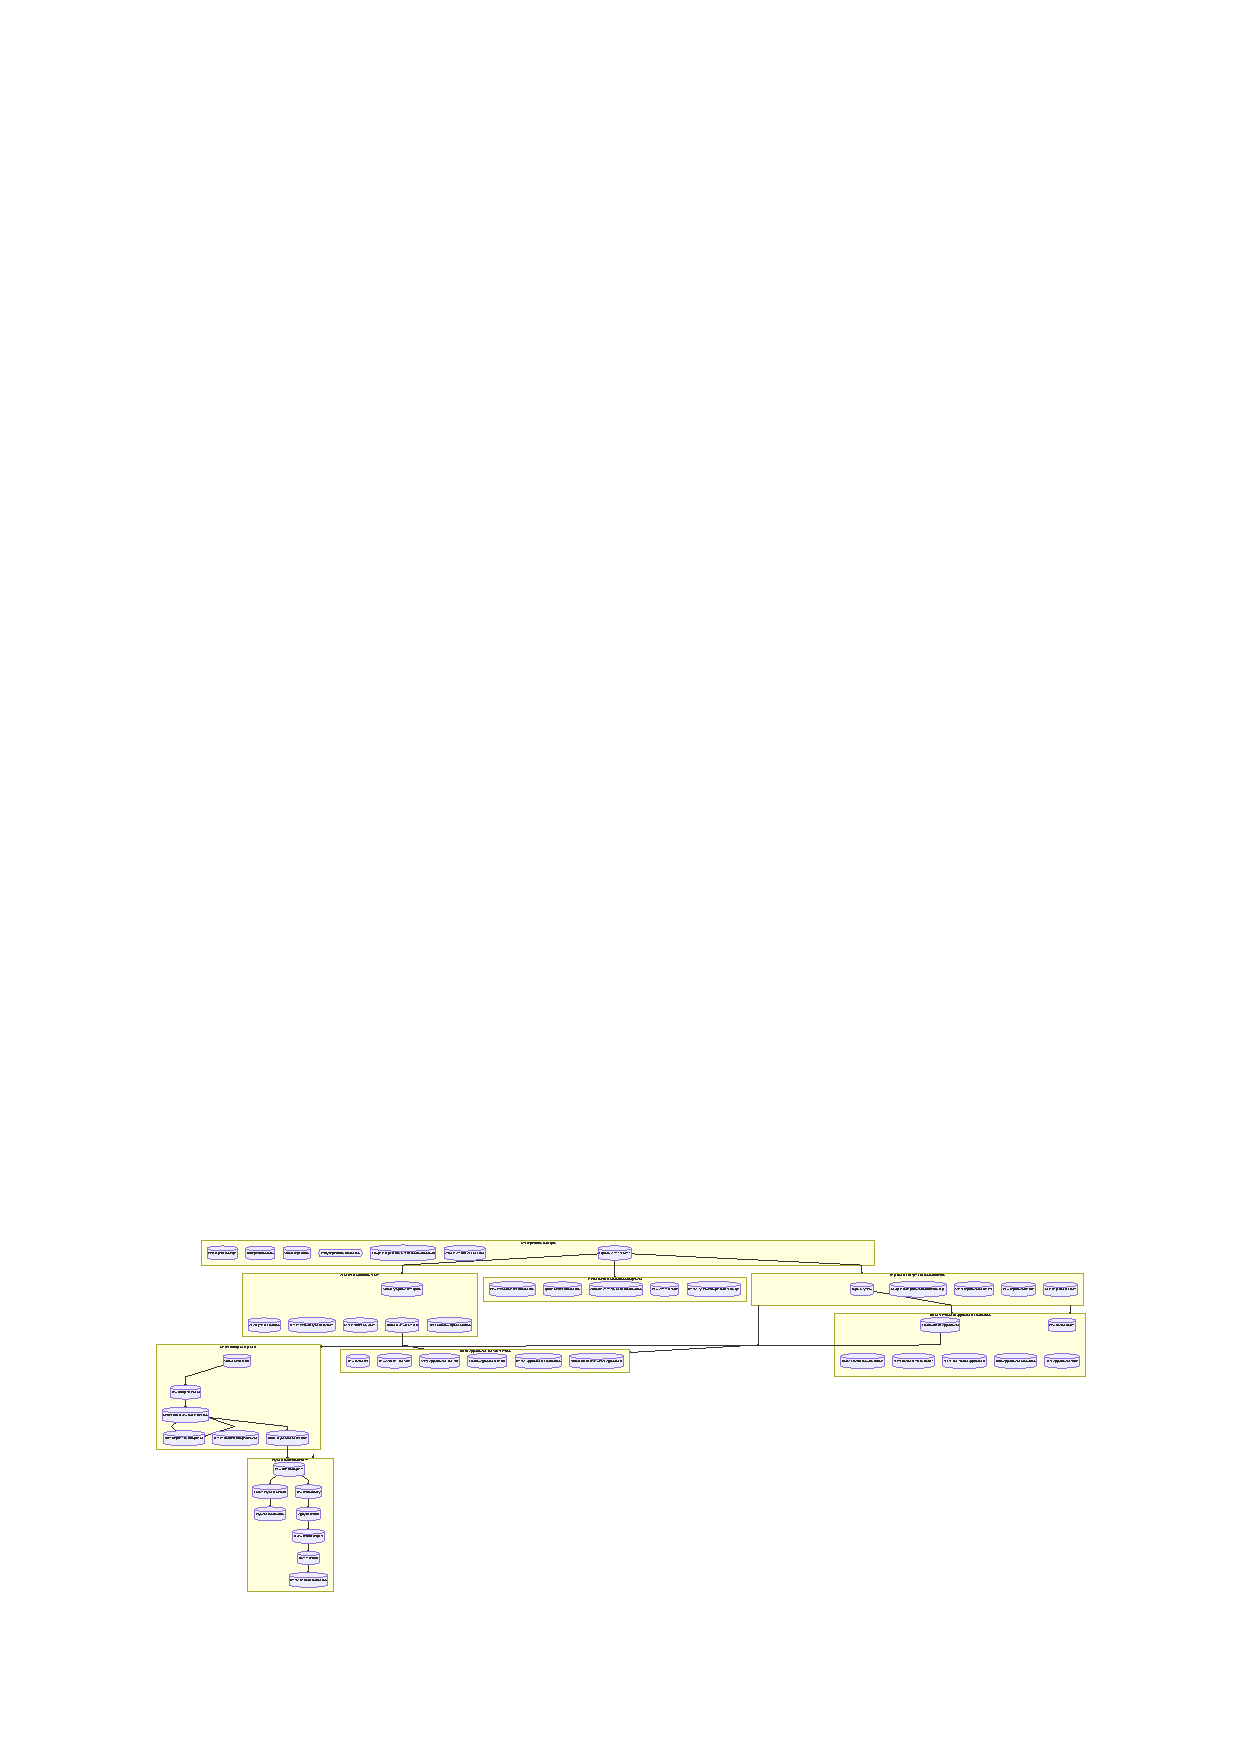
\includegraphics[width=0.9\textheight]{figures/01.pdf}}
	\caption{顶层数据流图}
\end{figure}
%%----------- 参考文献 -------------------%%
%在reference.bib文件中填写参考文献,此处自动生成

\reference


\end{document}